%! TEX root = main.tex

\graphicspath{{00_Images/02_chapter/}}

\chapter{Pre-amplification Stage}

The pre-amplification stage occupies the first active position in any audio signal chain, sitting immediately after the transducer in the typical path microphone \(\to\) pre-amplifier \(\to\) power amplifier \(\to\) loudspeaker. Its primary function is to raise the signal level to a usable range, preserve signal integrity across the audio band and minimize the loading effect on the source. Loading occurs whenever the input impedance of the amplifier is insufficiently large relative to the source impedance, causing a voltage divider to attenuate the signal before any processing takes place. Referring to the basic voltage divider formed by the source impedance \( Z_s \) and the amplifier input impedance \( Z_{in} \):
\[
V_{in} = V_s \cdot \frac{Z_{in}}{Z_s + Z_{in}}
\]
the ideal condition is \( Z_{in} \to \infty \), so that \( V_{in} \to V_s \) and the full source voltage is transferred without attenuation. In the opposite limit \( Z_{in} \to 0 \), the signal is completely suppressed. Maximizing \( Z_{in} \) is therefore the central design requirement for the input stage.

\section{Input Impedances and the Two-Port Model}
\label{sc:21}

\begin{figure}[!htb]
    \centering
    \subfloat{\includegraphics[width=0.47\linewidth]{Datasheet1.png}}
    \hfill
    \subfloat{\includegraphics[width=0.47\linewidth]{Datasheet2.png}}
    \caption{Excerpt from the Texas Instruments OPA1622 datasheet. The differential impedance \(Z_D \approx \SI{60}{\kilo\ohm}\) and the common-mode impedance \(Z_{CM} \approx \SI{500}{\mega\ohm}\) differ by four orders of magnitude, directly motivating the two-port input model}
    \label{fig:datasheetCMD}
\end{figure}

A rigorous treatment of the pre-amplifier input starts from real device parameters. The datasheet of the Burr-Brown OPA1622 (Texas Instruments), a high-performance audio Op-Amp representative of professional equipment, is used as the reference (figure \ref{fig:datasheetCMD}). Two entries are immediately relevant:

\begin{itemize}
    \item Differential input impedance \( Z_D \approx \SI{60}{\kilo\ohm} \), defined between the non-inverting (\(v^{+}\)) and inverting (\(v^{-}\)) terminals.
    \item Common-mode input impedance \( Z_{CM} \approx \SI{500}{\mega\ohm} \), defined between each input terminal and the internal reference.
\end{itemize}

The ratio \( Z_{CM}/Z_D \approx 8 000 \) reflects the internal topology of the differential input pair. A further feature of the datasheet is a capacitor listed in parallel with each impedance entry: at low and medium audio frequencies the capacitive branch is essentially open-circuit and the impedances behave resistively; at high frequencies the capacitive reactance decreases, the input impedance falls and the loading on the source increases.

\subsection{Why a Single-Impedance Model is Insufficient}

The simplest model for the Op-Amp input treats it as a single impedance \( Z_{in} \) shunted from the non-inverting terminal to ground. This representation is adequate only in purely single-ended configurations, where the inverting terminal is permanently at ground and the signal is applied solely to \( v^{+} \). It fails as soon as a non-zero voltage appears simultaneously on both input pins: a single shunt impedance predicts zero absorbed current whenever \( v^{+} = v^{-} \). In real devices, a finite current flows from each terminal toward the internal reference even in that condition, owing to the finite \( Z_{CM} \). Ignoring this current yields incorrect predictions of loading in balanced configurations.

\begin{figure}[!htb]
    \centering
    \subfloat[Basic Op-Amp symbol: the output is a function of the differential input, \( v_{out} = g(v^{+} - v^{-}) \)]{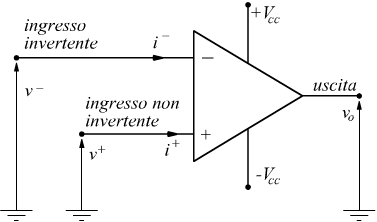
\includegraphics[height=0.22\textheight]{OpAmps.png}}
    \hfill
    \subfloat[Two-port input model: \( Z_D \) (\( R_{id} \) in scheme) between the differential terminals, \( Z_{CM}^{+} \) and \( Z_{CM}^{-} \) (\( R_{ic} \) in scheme) from each terminal to ground]{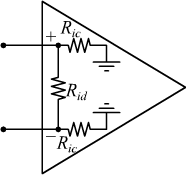
\includegraphics[height=0.22\textheight]{OpAmpImps.png}}
    \caption{Op-Amp representation. The single-impedance model implicit in the left symbol is replaced by the two-port network on the right, which captures both differential and common-mode loading correctly}
    \label{fig:oaScheme}
\end{figure}

The correct representation is the two-port input model of figure \ref{fig:aopEquivScheme}, comprising:

\begin{itemize}
    \item Differential impedance \( Z_D \): connected between \( v^{+} \) and \( v^{-} \); it loads the difference of the two input voltages.

    \item Common-mode impedances \( Z_{CM}^{+} \) and \( Z_{CM}^{-} \): connected from \( v^{+} \) and \( v^{-} \) to ground, respectively. They account for the current drawn even when both inputs carry the same signal. In a symmetric device \( Z_{CM}^{+} = Z_{CM}^{-} \).
\end{itemize}

\begin{figure}[!htb]
    \centering
    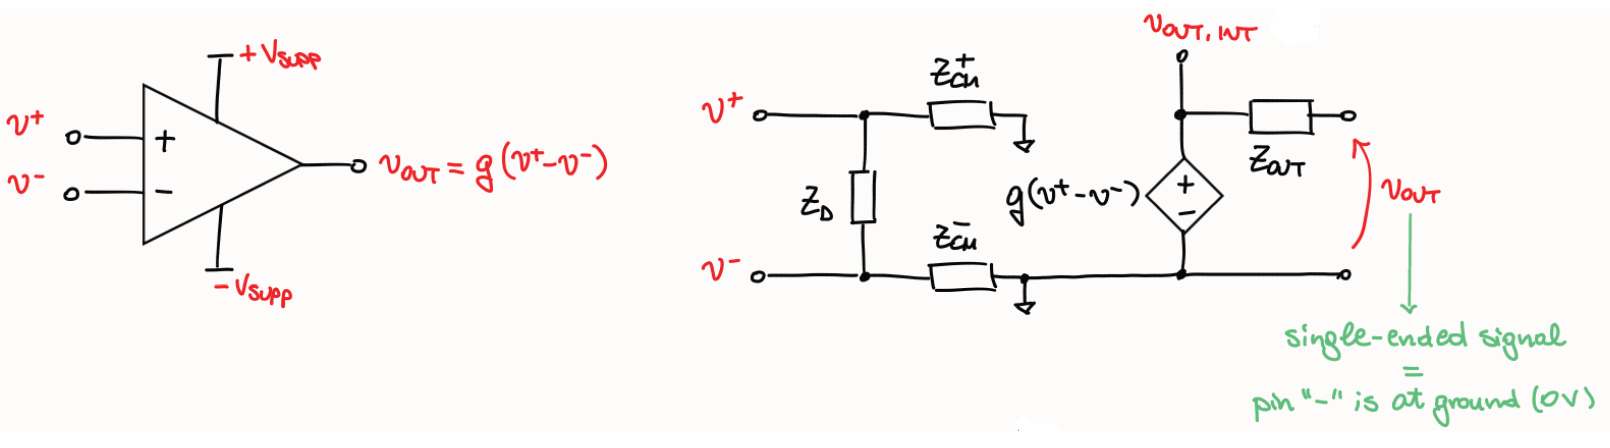
\includegraphics[width=0.90\textwidth]{AOP_equiv_scheme.png}
    \caption{Complete equivalent circuit of a real Op-Amp. The two-port input network contains \( Z_D \) between the differential terminals and \( Z_{CM}^{+} \), \( Z_{CM}^{-} \) to ground. The output stage is modeled as a voltage-controlled source \( g(v^{+}-v^{-}) \) driving through the output impedance \( Z_{out} \). The annotation single-ended signal indicates that the simplified single-port model is recovered only when pin ``\(-\)'' is held at \SI{0}{\volt}}
    \label{fig:aopEquivScheme}
\end{figure}

\section{Unbalanced Mode}

In the unbalanced (single-ended) configuration the source signal is applied only to the non-inverting terminal and the inverting terminal is tied to ground:
\[
v^{+} = v_{TEST}, \qquad v^{-} = 0
\]
This is the connection scheme of most consumer audio equipment (RCA, TS jack connectors). The circuit used to evaluate the input impedance is shown in figure \ref{fig:unbalancedConfig}.

\begin{figure}[!htb]
    \centering
    \subfloat[Unbalanced connection: signal on \( v^{+} \), \( v^{-} \) to ground]{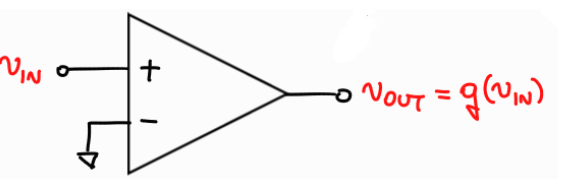
\includegraphics[height=0.12\textheight]{OPAMP_Unbalanced_config.png}}
    \hfill
    \subfloat[Test-source method: \( v_{TEST} \) is applied and the total current \( i_{TEST} \) is computed. The \( v^{-} \) branch is grounded on both ends and carries no current]{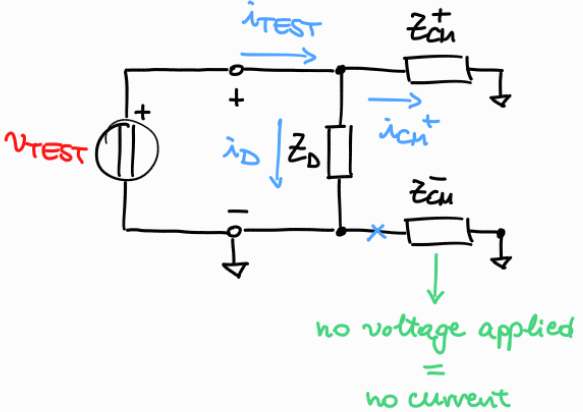
\includegraphics[height=0.17\textheight]{OPAMP_Unbalanced_Impedance_Eval.png}}
    \caption{Unbalanced input configuration and equivalent circuit for the input-impedance derivation via the test-source method}
    \label{fig:unbalancedConfig}
\end{figure}

\subsection{Input Impedance Derivation}

Two branches absorb current from the test source. The differential branch carries:
\[
i_D = \frac{v^{+} - v^{-}}{Z_D} = \frac{v_{TEST}}{Z_D}
\]
The upper common-mode branch draws:
\[
i_{CM}^{+} = \frac{v^{+}}{Z_{CM}^{+}} = \frac{v_{TEST}}{Z_{CM}^{+}}
\]
The lower common-mode branch \( Z_{CM}^{-} \) has \( v^{-}=0 \) on both terminals and therefore carries no current. Applying KCL at the \( v^{+} \) node:
\[
i_{TEST} = i_D + i_{CM}^{+}= v_{TEST}\left(\frac{1}{Z_D} + \frac{1}{Z_{CM}^{+}}\right)
\]
The input impedance follows directly:
\[
Z_{in}^{UNB}= \frac{v_{TEST}}{i_{TEST}}= Z_D  ||  Z_{CM}^{+}= \frac{Z_D  Z_{CM}^{+}}{Z_D + Z_{CM}^{+}}
\]
With \( Z_{CM}^{+} \approx \SI{500}{\mega\ohm} \gg Z_D \approx \SI{60}{\kilo\ohm} \), the parallel combination is dominated by the smaller term and \( Z_{in}^{UNB} \approx Z_D \). This confirms that the differential impedance entry of the datasheet is precisely the unbalanced input impedance at audio frequencies.

\section{Balanced Mode}

In the balanced configuration both input terminals carry signals and the device operates as a differential amplifier producing \( v_{out} = g(v_1 - v_2) \), as shown in figure \ref{fig:balancedConfig}. This is the connection scheme of professional audio (XLR, TRS balanced connectors).

\begin{figure}[!htb]
    \centering
    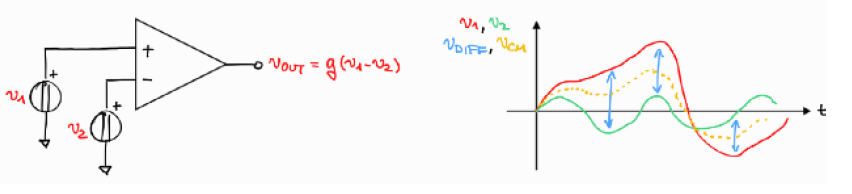
\includegraphics[width=0.90\textwidth]{OPAMP_Balanced_Config.png}
    \caption{Balanced input configuration (left) and representative time-domain waveforms (right). The two line voltages \( v_1 \) and \( v_2 \) carry the audio information encoded as their difference \( v_{DIFF} \) (blue), while the common-mode component \( v_{CM} \) (yellow dashed) represents coupled interference that the differential stage rejects}
    \label{fig:balancedConfig}
\end{figure}

\subsection{Signal Decomposition}
\label{sc:231}

Any pair of terminal voltages \( (v_1, v_2) \) is uniquely decomposed into a common-mode and a differential component:
\[
v_{DIFF} = v_1 - v_2
\qquad \text{(zero-average: carries the audio signal)}
\]
\[
v_{CM} = \frac{v_1 + v_2}{2}
\qquad \text{(average: carries interference)}
\]
The inverse transformation recovers each terminal voltage from the two components:
\[
v_1 = v_{CM} + \frac{v_{DIFF}}{2},
\qquad
v_2 = v_{CM} - \frac{v_{DIFF}}{2}
\]

Two limiting excitation cases are physically important.

\paragraph{Pure differential excitation with \( v_{CM} = 0 \)} Both terminals are driven symmetrically with opposite signs:
\[
v_1 = +\frac{v_{DIFF}}{2}, \qquad v_2 = -\frac{v_{DIFF}}{2}
\]

\paragraph{Pure common-mode excitation with \( v_{DIFF} = 0 \)} Both terminals carry the same potential:
\[
v_1 = v_2 = v_{CM}
\]
The general balanced excitation (figure \ref{fig:diffCMmodes}) is the superposition of these two cases.

\begin{figure}[!htb]
    \centering
    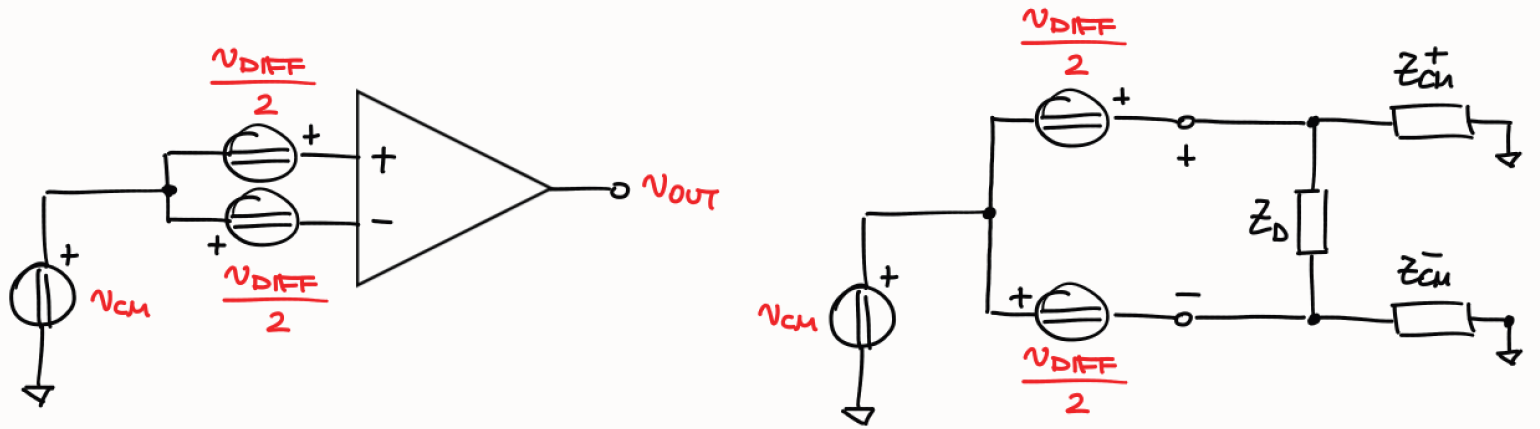
\includegraphics[width=0.90\textwidth]{OPAMP_Diff_Common_modes.png}
    \caption{General balanced excitation decomposed into a pure differential source \( \pm v_{DIFF}/2 \) and a pure common-mode source \( v_{CM} \) in series. The two-port input network shows the physical paths followed by the differential current (through \( Z_D \)) and the common-mode current (through \( Z_{CM}^{+} \) and \( Z_{CM}^{-} \))}
    \label{fig:diffCMmodes}
\end{figure}

\subsection{Pure Differential Mode: Differential Input Impedance}

The differential input impedance is defined at zero common-mode excitation:
\[
Z_{DIFF} = \left.\frac{v_{DIFF}}{i_{DIFF}}\right|_{v_{CM}=0}
\]
With \( v^{+} = v_{DIFF}/2 \) and \( v^{-} = -v_{DIFF}/2 \), the current entering the \( v^{+} \) terminal is (figure \ref{fig:pureDiff}):
\[
i_{DIFF}= \frac{v^{+} - v^{-}}{Z_D} + \frac{v^{+}}{Z_{CM}^{+}}= \frac{v_{DIFF}}{Z_D} + \frac{v_{DIFF}}{2 Z_{CM}^{+}}
\]
Substituting yields:
\[
Z_{DIFF} = \frac{v_{DIFF}}{i_{DIFF}} = Z_D  ||  2Z_{CM}^{+} = \frac{2 Z_D Z_{CM}^{+}}{Z_D + 2 Z_{CM}^{+}}
\]
Since \( Z_{CM}^{+} \gg Z_D \), it follows that \( Z_D \ll 2Z_{CM}^{+} \) and therefore \( Z_{DIFF} \approx Z_D \), consistent with the datasheet value.

\subsection{Pure Common Mode: Common-Mode Input Impedance}

The common-mode input impedance is defined at zero differential excitation:
\[
Z_{CM} = \left.\frac{v_{CM}}{i_{CM}}\right|_{v_{DIFF}=0}
\]
With \( v^{+} = v^{-} = v_{CM} \), no voltage appears across \( Z_D \) and that branch draws no current. The total source current flows entirely through the two common-mode branches in parallel (figure \ref{fig:pureCM}):
\[
i_{CM} = \frac{v_{CM}}{Z_{CM}^{+}} + \frac{v_{CM}}{Z_{CM}^{-}} = v_{CM}\left(\frac{1}{Z_{CM}^{+}} + \frac{1}{Z_{CM}^{-}}\right)
\]
Therefore:
\[
Z_{CM} = Z_{CM}^{+}  ||  Z_{CM}^{-} = \frac{Z_{CM}^{+} Z_{CM}^{-}}{Z_{CM}^{+}+Z_{CM}^{-}}
\]
For a symmetric device \( Z_{CM}^{+} = Z_{CM}^{-} = Z_{CM,0} \), this yields \( Z_{CM} = Z_{CM,0}/2 \approx \SI{250}{\mega\ohm} \), confirming the very high common-mode impedance indicated in the datasheet.

\begin{figure}[!htb]
    \centering
    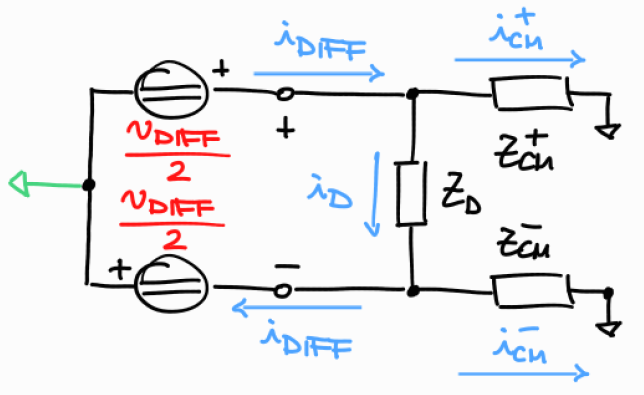
\includegraphics[width=0.7\textwidth]{OPAMP_pure_differential_scheme.png}
    \caption{Pure differential excitation of the two-port input model. Each terminal is driven by a source of magnitude \( v_{DIFF}/2 \) with opposite polarity. The differential current \( i_{DIFF} \) splits between \( Z_D \), \( Z_{CM}^{+} \) and \( Z_{CM}^{-} \)}
    \label{fig:pureDiff}
\end{figure}

\begin{figure}[!htb]
    \centering
    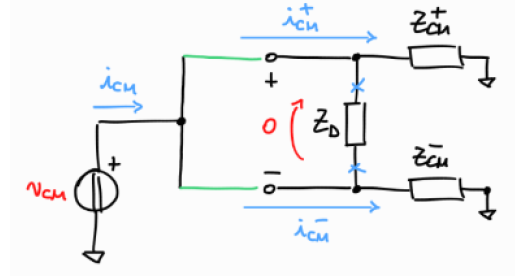
\includegraphics[width=0.7\textwidth]{OPAMP_pure_common_mode_scheme.png}
    \caption{Pure common-mode excitation of the two-port input model. Both terminals are driven to \( v_{CM} \); the differential impedance \( Z_D \) (marked with a zero voltage drop) carries no current. All of \( i_{CM} \) flows through the parallel combination of \( Z_{CM}^{+} \) and \( Z_{CM}^{-} \), yielding \( Z_{CM} = Z_{CM}^{+} || Z_{CM}^{-} \)}
    \label{fig:pureCM}
\end{figure}

\section{Gain Models}

The pre-amplifier is treated as a linear time-invariant (LTI) system in its linear operating region. A general two-port LTI block relates input quantities \( (V, I, Q, \ldots) \) to output quantities \( Y \) through a gain function. Depending on the port variables of interest, three distinct gain figures are defined.

\begin{itemize}
    \item Voltage gain:
    \[
    G_V = \frac{V_{out}}{V_{in}} > 1,
    \qquad
    G_{V,\mathrm{dB}} = 20\log_{10}\left(G_V\right)
    \]
    \item Current gain:
    \[
    G_I = \frac{I_{out}}{I_{in}} > 1,
    \qquad
    G_{I,\mathrm{dB}} = 20\log_{10}\left(G_I\right)
    \]
    \item Power gain:
    \[
    G_P = \frac{P_{out}}{P_{in}} > 1,
    \qquad
    G_{P,\mathrm{dB}} = 10\log_{10}\left(G_P\right)
    \]
    The factor of 10 (not 20) in the power dB conversion reflects the fact that power is proportional to the square of voltage or current.
\end{itemize}

The corresponding attenuation factors are the reciprocals of the respective gains:
\[
A_{tt,V} = \frac{V_{in}}{V_{out}} = \frac{1}{G_V},
\qquad
A_{tt,V}|_{\mathrm{dB}} = 20\log_{10}\left(\frac{1}{G_V}\right) = -G_{V,\mathrm{dB}}
\]
and analogously for the current attenuation \( A_{tt,I} = 1/G_I \).

\subsection{Buffer Configurations}

Three special cases of the gain definitions are of particular practical importance in audio pre-amplification.

\paragraph{Voltage buffer} The voltage gain is unity but, with a very high input impedance (\( Z_{in} \to \infty \)), virtually no input current is drawn from the source. The output can supply the full load current, yielding \( G_V = 1 \), \( G_I > 1 \), \( G_P > 1 \). This configuration solves the impedance mismatch: a source with high \( Z_S \) would lose virtually all its signal into a low-impedance load without buffering, while a buffer with \( Z_{in} \to \infty \) transfers the full source voltage to the output irrespective of the load.

\paragraph{Current buffer} The current gain is unity while voltage and power gains can exceed unity: \( G_I = 1 \), \( G_V > 1 \), \( G_P > 1 \). The current buffer preserves the signal current while transforming the impedance level.

\paragraph{Remark on attenuation} If \( G_V < 1 \), the stage attenuates the signal rather than amplifying it. In dB notation \( G_{V,\mathrm{dB}} < 0 \) and the attenuation value \( A_{tt,V}|_{\mathrm{dB}} = -G_{V,\mathrm{dB}} > 0 \).

\section{Frequency Response and Dynamic Range}
\label{sc:25}

\subsection{Frequency-Dependent Gain}

The voltage gain \( G_V \) of a real pre-amplifier is not constant across frequency. Figure \ref{fig:preampFreqResp} shows a representative Bode magnitude plot: the gain is approximately flat within the audio passband (e.g. \SI{20}{\decibel} \(= \times 10\) at \SI{100}{\hertz}), then rolls off toward high frequencies due to capacitive parasitics internal to the device. The same gain is defined as the slope of the transfer characteristic in the linear region of the \( V_{out} \) vs. \( V_{in} \) plot: measuring this ratio at different test frequencies (e.g. \SI{100}{\hertz} vs. \SI{10}{\kilo\hertz}) reveals the passband value and the roll-off separately.

\begin{figure}[!htb]
    \centering
    \subfloat{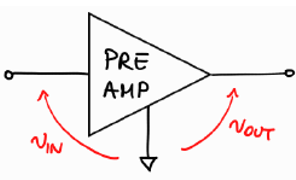
\includegraphics[width=0.3\linewidth]{Basic_Pre_Amp.png}}
    \\
    \subfloat{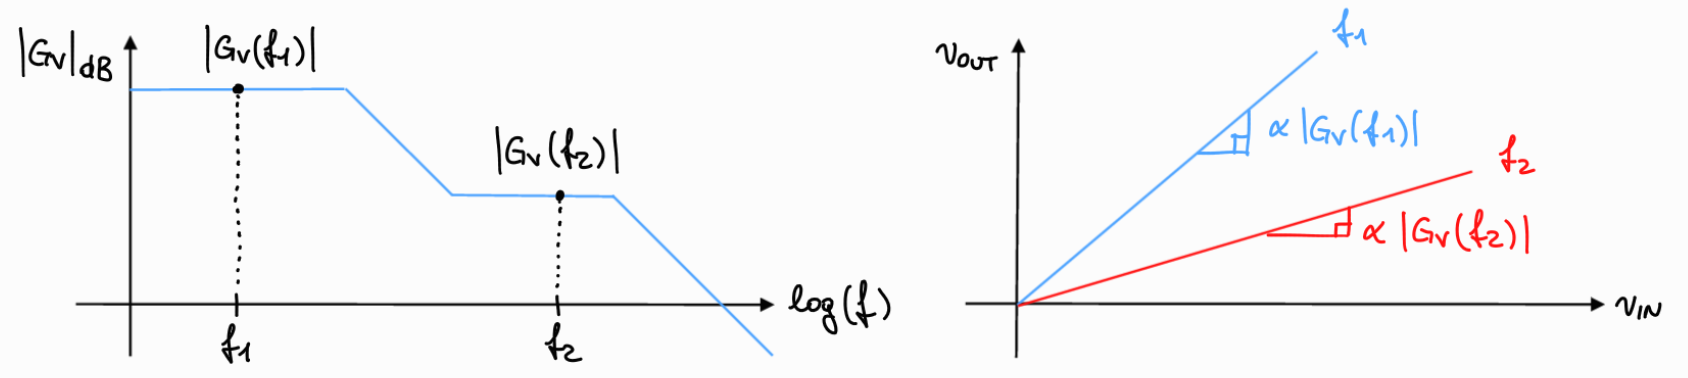
\includegraphics[width=0.9\linewidth]{PreAmp_Freq_Resp.png}}
    \caption{Basic pre-amplifier block (left) and its frequency response (right). The Bode magnitude plot shows a flat passband (\SI{20}{\decibel} at \SI{100}{\hertz}) followed by a high-frequency roll-off above \SI{1}{\kilo\hertz}. The \( V_{out} \) vs. \( V_{in} \) characteristic on the right has a slope equal to \( G_V \) evaluated at the corresponding test frequency}
    \label{fig:preampFreqResp}
\end{figure}

\subsection{Power Supply and Saturation}

A pre-amplifier is not an energy source: to amplify a signal it draws power from an external supply \( V_{SUPP} \), as shown in figure \ref{fig:powerSupply}. The power budget at the output port is:
\[
P_{out} = P_{in} + P_G, \qquad P_{out} > P_{in}
\]
where \( P_G \) is the power drawn from the supply (\( P_{SUPP} = V_{SUPP}\cdot I_{SUPP} \)).

\begin{figure}[!htb]
    \centering
    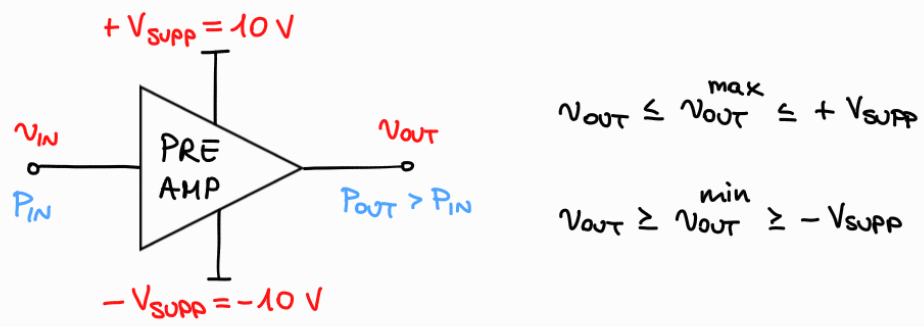
\includegraphics[width=0.55\textwidth]{PreAmp_Power_Supply.png}
    \caption{Pre-amplifier powered by a supply \( V_{SUPP} \). The output power \( P_{out} \) exceeds the input power \( P_{in} \) by \( P_G \) drawn from the supply, confirming \( P_{out} > P_{in} \)}
    \label{fig:powerSupply}
\end{figure}

The output voltage is bounded by the supply rails: \( |V_{out}| \leq V_{out}^{\max} \), where in practice \( V_{SUPP} > V_{out}^{\max} \) due to internal headroom losses. When the required output exceeds \( V_{out}^{\max} \), the amplifier saturates and the waveform clips. The lower usable limit is set by the noise floor \( V_{out}^{\min} \): signals below this level are masked by thermal and device noise and cannot be reliably amplified.

\subsection{Dynamic Range}
\label{ssc:253}

The dynamic range (DR) quantifies the ratio between the maximum and minimum usable signal levels. Two complementary figures are defined:

\[
DR^{OUT} = \frac{V_{out}^{\max}}{V_{out}^{\min}},
\qquad
DR^{IN} = \frac{V_{in}^{\max}}{V_{in}^{\min}}
\]
In the linear operating region these are related by the voltage gain:
\[
DR^{IN} = \frac{DR^{OUT}}{G_V}
\]
For a fixed supply (fixed \( V_{out}^{\max} \)), increasing the gain reduces the maximum allowable input before saturation:
\[
\begin{cases}
    G_V = 1   & \Rightarrow\; DR^{IN} = DR^{OUT}    \\
    G_V = 10  & \Rightarrow\; DR^{IN} = DR^{OUT}/10 \\
    G_V = 100 & \Rightarrow\; DR^{IN} = DR^{OUT}/100
\end{cases}
\]

\begin{figure}[!htb]
    \centering
    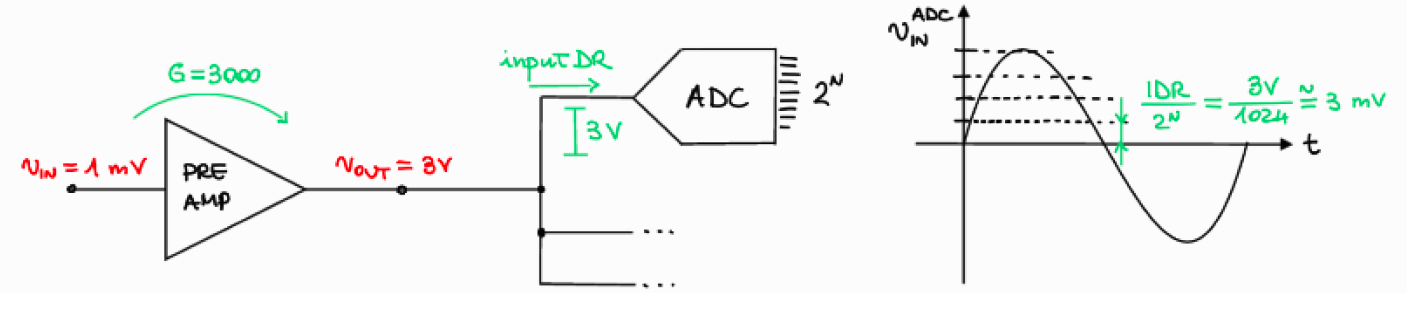
\includegraphics[width=0.90\textwidth]{Dynamic_Range_with_ADC.png}
    \caption{Dynamic range of the pre-amplifier stage. The output is bounded above by the supply-limited clipping level \( V_{out}^{\max} \) and below by the noise floor \( V_{out}^{\min} \). Higher gain \( G_V \) compresses the input dynamic range \( DR^{IN} = DR^{OUT}/G_V \) proportionally, increasing susceptibility to overload}
    \label{fig:dynamicRange}
\end{figure}

\subsection{Spurious-Free Dynamic Range}

When the output signal approaches \( V_{out}^{\max} \), the amplifier exhibits non-linear behavior before hard clipping occurs. Non-linearity generates harmonic distortion: a sinusoidal input at fundamental frequency \( f_0 \) produces spurious output components at \( 2f_0, 3f_0, 4f_0,\ldots \), visible above the noise floor in the output spectrum. The Spurious-Free Dynamic Range (SFDR) is defined as the ratio between the fundamental and the largest spurious harmonic:
\[
\mathrm{SFDR} = \frac{|S(f_0)|}{|S(f_{spur})|_{\max}}
\]
SFDR is a more stringent quality figure than DR because it accounts for the harmonic content generated at high signal levels, where a DR calculation alone would still indicate an acceptable operating point.

\section{Distortion, Soft Knee, THD, IMD and SFDR}

Even before the output reaches the hard-clipping boundary at \( V_{out}^{\max} \), a real amplifier exhibits a gradual compression of signal peaks. This smooth transition from the linear region to limiting is called the soft knee: the transfer characteristic bends, producing spurious spectral components that grow in amplitude as the input level increases. The soft knee can be described systematically by expanding the output as a power series around the operating point, including a DC offset \( G_0 \) and keeping terms up to an arbitrary order \( N \):
\[
v_{out} = g(v_{in}),
\qquad
v_{out} = G_0 + \sum_{n=1}^{N} G_n   v_{in}^{n}
\]
Expanding the summation and grouping terms by their physical role:
\[
v_{out} = \underbrace{G_0}_{\text{DC offset}}
        + \underbrace{G_1 v_{in}}_{\text{linear (desired)}}
        + \underbrace{G_2 v_{in}^{2} + G_3 v_{in}^{3} + \cdots}_{\text{non-linear (distortion)}}
\]
The first two terms reproduce the ideal LTI behavior. The higher-order terms are responsible for all distortion phenomena: they are small for small \( v_{in} \) and grow rapidly as the input approaches the headroom limit, which is why distortion is strongly amplitude-dependent.

\subsection{Harmonic Generation and THD}

To understand the spectral consequence of the quadratic term, let the input be a single sinusoid:
\[
v_{in}(t) = V_{in}\sin(\omega_{in} t)
\]
Retaining the linear and quadratic terms of the power series:
\[
v_{out}(t) = G_1 V_{in}\sin(\omega_{in} t) + G_2 V_{in}^{2}\sin^{2}(\omega_{in} t)
\]
Squaring the sine doubles the frequency and creates a DC component. Using the identity \( \sin^2(\theta) = \tfrac{1}{2}(1 - \cos 2\theta) \):
\[
v_{out}(t) = \frac{G_2}{2}V_{in}^2
             + G_1 V_{in}\sin(\omega_{in} t)
             - \frac{G_2}{2}V_{in}^2\cos(2\omega_{in} t)
\]
The output therefore contains three components: a DC shift proportional to \( V_{in}^2 \), the desired fundamental at \( \omega_{in} \) and an unwanted second harmonic at \( 2\omega_{in} \). Accounting for all higher-order terms, the general output is a sum of harmonics (phases omitted for conciseness):
\[
v_{out}(t) = \sum_{i=1}^{N} v_{out,i}\sin(i \omega_{in} t)
= v_{out,1}\sin(\omega_{in} t) + v_{out,2}\sin(2\omega_{in} t) + \cdots
\]
Only the fundamental \( v_{out,1} \) is desired; all remaining components constitute harmonic distortion. The distortion factor of the \( i \)-th harmonic is defined as:
\[
D_i = \frac{v_{out,i}}{v_{out,1}}
\]
Considering a general load \( R_L \), the mean power of the \( i \)-th component is
\( P_i = v_{out,i}^2 / (2R_L) \), so the total output power is:
\[
\overline{P}_{out} = \frac{v_{out,1}^2 + v_{out,2}^2 + \cdots + v_{out,N}^2}{2R_L}
= \overline{P}_1 \left(1 + D_2^2 + \cdots + D_N^2\right),
\qquad \overline{P}_1 = \frac{v_{out,1}^2}{2R_L}
\]
The Total Harmonic Distortion is then defined as:
\[
\mathrm{THD} = \sqrt{D_2^2 + D_3^2 + \cdots + D_N^2}
\]

\paragraph{Amplitude dependence} THD is negligibly small in the linear regime of small \( v_{in} \), where the higher-order coefficients \( G_2, G_3, \ldots \) contribute negligibly. As \( v_{in} \) grows toward \( V_{in}^{\max} \), the non-linear terms grow faster than the linear term (quadratic, cubic, \ldots), causing THD to rise sharply. This is the essential physical reason why THD is reported in datasheets at a specified input level and supply voltage: both conditions set the operating point relative to the soft-knee region.

\subsection{Intermodulation Distortion}

When the amplifier is driven by two simultaneous tones, it operates outside the linear regime and the superposition principle no longer holds:
\[
g\left(x_1(t) + x_2(t)\right) \neq g\left(x_1(t)\right) + g\left(x_2(t)\right)
\]
Consider an input composed of two sinusoids at frequencies \( f_1 \) and \( f_2 \):
\[
v_{in}(t) = V_1\sin(\omega_1 t) + V_2\sin(\omega_2 t)
\]
Retaining the linear and quadratic terms:
\[
v_{out}(t) = G_1 v_{in} + G_2 v_{in}^2
\]
Expanding and grouping contributions:

\begin{align*}
v_{out}(t) &= \underbrace{G_1 V_1\sin(\omega_1 t) + G_1 V_2\sin(\omega_2 t)}_{\text{linear terms}}\\
&+ \underbrace{G_2\left[V_1^2\sin^2(\omega_1 t) + V_2^2\sin^2(\omega_2 t)\right]}_{\text{harmonic terms}}\\
&+ \underbrace{2G_2 V_1 V_2\sin(\omega_1 t)\sin(\omega_2 t)}_{\text{IMD (second order)}}
\end{align*}

The cross-product term expands as \( 2\sin(\omega_1 t)\sin(\omega_2 t) = \cos\left[(\omega_1-\omega_2)t\right] - \cos\left[(\omega_1+\omega_2)t\right] \), generating new spectral lines at \( f_2 - f_1 \) and \( f_2 + f_1 \). These are the second-order intermodulation products. Higher-order terms produce third-order products at \( 2f_1 - f_2, 2f_2 - f_1, 2f_1 + f_2, 2f_2 + f_1 \) and so on. Third-order products are often the most problematic: the mixing frequencies \( 2f_1 - f_2 \) and \( 2f_2 - f_1 \) can fall inside the audio band even when \( f_1 \) and \( f_2 \) are high-frequency tones, making them indistinguishable from the original signal.

\paragraph{Intercept power} The intercept power (IP) is the extrapolated input level at which an intermodulation product would equal the fundamental in amplitude, assuming the device operates in the regime where the power-series model applies. It is not directly measurable but is widely used to rank devices and to predict overload behavior at high signal levels.

\subsection{SFDR}

The Spurious-Free Dynamic Range (SFDR) extends the dynamic-range concept of section \ref{ssc:253} by accounting explicitly for distortion in addition to the noise floor. It is defined as the ratio between the amplitude of the fundamental output component and the largest spurious spectral line, whether harmonic or intermodulation:
\[
\mathrm{SFDR} = \frac{|S(f_0)|}{|S(f_{spur})|_{\max}}
\]
SFDR is the more informative specification for audio quality because it captures the onset of non-linear behavior before hard clipping occurs.

\subsection{Audio Spectrum Splitting}

IMD is most severe when a single amplifier is required to handle tones spanning the full audio band simultaneously. The practical mitigation adopted in electroacoustic systems is to divide the audio spectrum into sub-bands, typically Low, Mid and High and route each sub-band to a dedicated amplification chain and transducer. The frequency splitting is performed by a set of crossover filters before the power amplifiers:

\begin{itemize}
    \item a low-pass filter (LPF) drives the woofer (\(\lesssim \SI{500}{\hertz}\));
    \item a band-pass filter (BPF) drives the mid-range driver (\(\SIrange{500}{5000}{\hertz}\));
    \item a high-pass filter (HPF) drives the tweeter (\(\gtrsim \SI{5}{\kilo\hertz}\)).
\end{itemize}

Each amplifier then operates over a reduced bandwidth, lowering the probability of generating in-band IMD products and allowing the transducer to be optimised for its specific frequency range.

\section{Non-Ideal Amplifiers: Gain Mismatch}

An ideal Op-Amp performs an exact subtraction: \( v_{out} = G(v^{+} - v^{-}) \). In practice, the two input terminals are processed by slightly different internal gain paths, so the general transfer function must be written as:
\[
v_{out} = G^{+} v^{+} - G^{-} v^{-}
\]
where \( G^{+} \) and \( G^{-} \) are individually defined (figure \ref{fig:gcmgdiff}) and are not necessarily equal.

\begin{figure}[!htb]
    \centering
    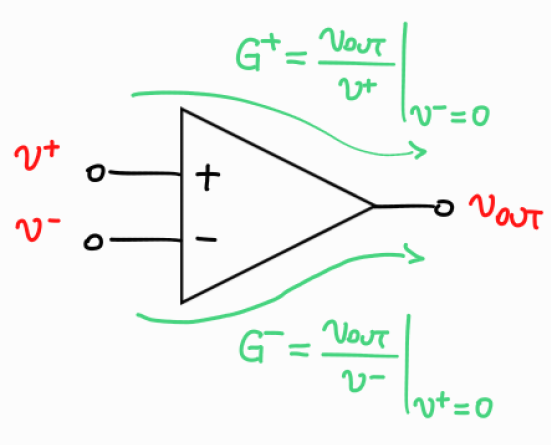
\includegraphics[width=0.90\textwidth]{OPAMP_G_CM_G_DIFF.png}
    \caption{Definition of the partial gains \( G^{+} = v_{out}/v^{+}|_{v^{-}=0} \) and \( G^{-} = v_{out}/v^{-}|_{v^{+}=0} \). Gain mismatch (\( G^{+} \neq G^{-} \)) is the origin of non-zero common-mode gain and finite CMRR in real differential amplifiers}
    \label{fig:gcmgdiff}
\end{figure}

Substituting the signal decomposition from equations of the beginning of this chapter, \( v^{+} = v_{CM} + v_{DIFF}/2 \) and \( v^{-} = v_{CM} - v_{DIFF}/2 \):
\[
v_{out} = G^{+}\left(v_{CM} + \frac{v_{DIFF}}{2}\right)
        - G^{-}\left(v_{CM} - \frac{v_{DIFF}}{2}\right)
\]
Collecting terms:
\[
v_{out} = \underbrace{\frac{G^{+} + G^{-}}{2}}_{G_{DIFF}} v_{DIFF}
        + \underbrace{\left(G^{+} - G^{-}\right)}_{G_{CM}} v_{CM}
\]
Two gain parameters emerge:
\[
G_{DIFF} = \frac{G^{+} + G^{-}}{2},
\qquad
G_{CM} = G^{+} - G^{-}
\]
so that the output is expressed compactly as:
\[
v_{out} = G_{DIFF}  v_{DIFF} + G_{CM}  v_{CM}
\]

\paragraph{Counterintuitive naming} The labeling is easily confused with the signal definitions. The gain \( G_{DIFF} \) that should amplify the wanted signal, is actually the average of the two individual gains. \( G_{CM} \), the gain that should ideally be zero, is actually the difference between the two gains. Consequently, a perfectly matched pair (\( G^{+} = G^{-} \)) yields \( G_{CM} = 0 \) and \( G_{DIFF} = G^{+} \), which is the ideal result. Any mismatch \( G^{+} \neq G^{-} \) immediately introduces a non-zero common-mode gain and degrades disturbance rejection.

\section{External Disturbances and CMRR}

Physical cables and connectors exposed to electromagnetic fields act as antennas. A transient disturbance in the environment, a power-line spike, a mechanical impulse on the cable or a nearby switching event, injects a voltage \( v_{DIST} \) into the signal path. The coupling mechanism is capacitive: the disturbing source and the cable conductor form a parasitic capacitor \( C_c \), through which a transient current flows. Modeling the coupling as a capacitor is physically motivated by the absence of a DC path between the disturber and the cable: only transient (AC) disturbances are transmitted, while steady-state offsets are blocked.

\subsection{Balanced Configuration}

In a balanced interconnection, the source signal \( v_s \) is conveyed as \( +v_s/2 \) on the hot conductor and \( -v_s/2 \) on the cold conductor. An external disturbance \( v_{DIST} \) couples through parasitic capacitors \( C_c \) onto both conductors simultaneously and with equal amplitude, making it a pure common-mode voltage. Figure \ref{fig:distBal} shows the complete circuit.

\begin{figure}[!htb]
    \centering
    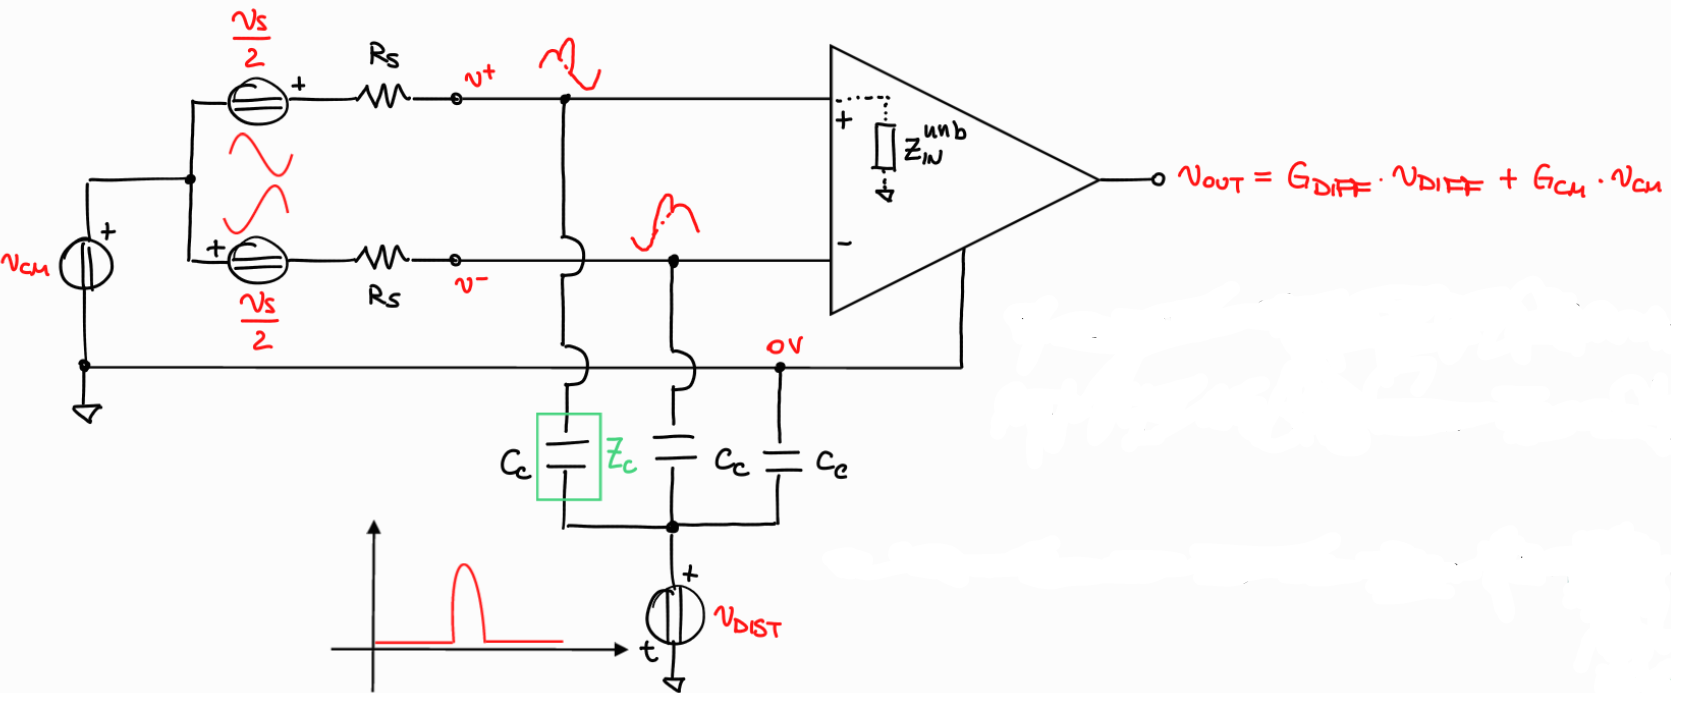
\includegraphics[width=0.90\textwidth]{OPAMP_Disturbances_Balanced.png}
    \caption{Balanced configuration with a common-mode disturbance \( v_{DIST} \) coupled through parasitic capacitors \( C_c \) onto both conductors. At the amplifier input: \( v_{DIFF} = v^{+} - v^{-} = v_s \) and \( v_{CM} = v_{DIST} \), so the output is \( v_{out} = G_{DIFF}  v_s + G_{CM}  v_{DIST} \)}
    \label{fig:distBal}
\end{figure}

At the amplifier input terminals:
\[
v_{DIFF} = v^{+} - v^{-}
= \left(\frac{v_s}{2} + v_{DIST}\right) - \left(-\frac{v_s}{2} + v_{DIST}\right)
= v_s
\]
\[
v_{CM} = \frac{v^{+} + v^{-}}{2} = v_{DIST}
\]
The output is therefore:
\[
v_{out} = G_{DIFF}  v_s + G_{CM}  v_{DIST}
= G_{DIFF}\left(v_s + \frac{G_{CM}}{G_{DIFF}} v_{DIST}\right)
\]
When \( G_{CM} \ll G_{DIFF} \), the disturbance is strongly attenuated relative to the signal.

\subsection{Unbalanced Configuration}

In an unbalanced connection the signal is referenced to ground, so \( v^{-} = 0 \) and any disturbance that reaches the input is indistinguishable from the signal. Figure \ref{fig:distUnbal} illustrates the coupling path.

\begin{figure}[!htb]
    \centering
    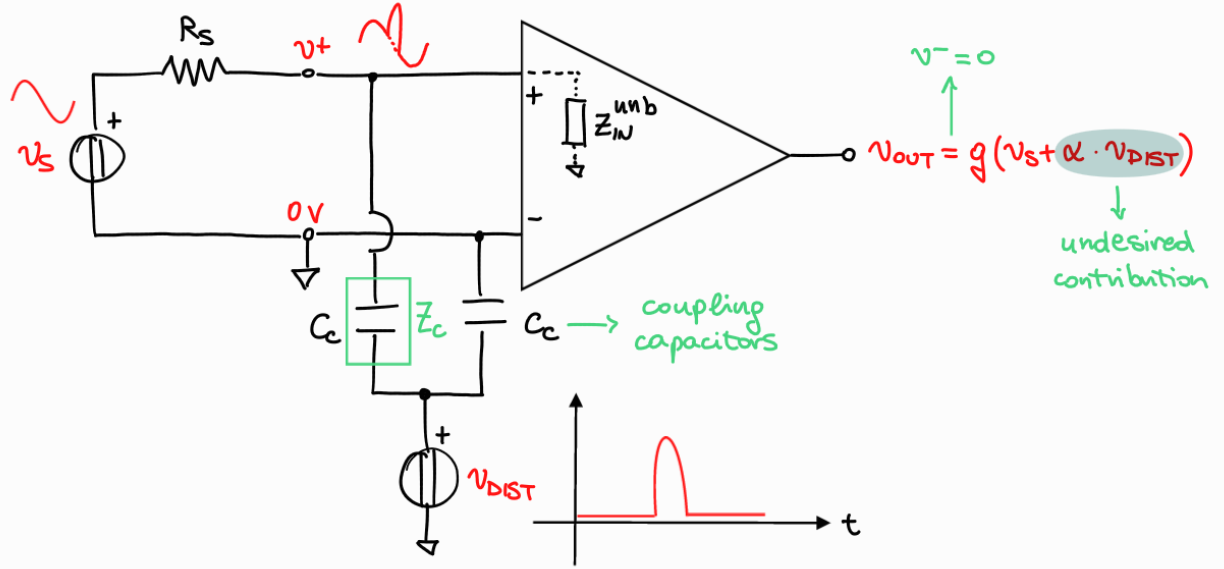
\includegraphics[width=0.90\textwidth]{OPAMP_Disturbances_Unbalanced.png}
    \caption{Unbalanced configuration with a disturbance \( v_{DIST} \) coupled through the cable impedance \( Z_C \) and parasitic capacitors \( C_c \). Setting \( v_s = 0 \), the disturbance reaches \( v^{+} \) through the divider \( Z_{eq} / (Z_{eq} + Z_C) \) with \( Z_{eq} = R_s  ||  Z_{in}^{UNB} \). The amplified output is \( v_{out} = g(v_s + \alpha  v_{DIST}) \)}
    \label{fig:distUnbal}
\end{figure}

Setting \( v_s = 0 \) to isolate the disturbance contribution:
\[
v^{+} = v_{DIST} \cdot \frac{Z_{eq}}{Z_{eq} + Z_C},
\qquad Z_{eq} = R_s  ||  Z_{in}^{UNB}
\]
The disturbance is transferred through a voltage divider that depends on the impedance of the source, the cable coupling impedance and the amplifier input impedance. Unlike the balanced case, there is no cancellation mechanism: the disturbance enters the signal path directly through the single input conductor.

\subsection{Common-Mode Rejection Ratio}

The quality of disturbance rejection in a differential stage is quantified by the Common-Mode Rejection Ratio:
\[
\mathrm{CMRR} = \left|\frac{G_{DIFF}}{G_{CM}}\right|,
\qquad
\mathrm{CMRR}_{dB} = 20\log_{10}\left(\left|\frac{G_{DIFF}}{G_{CM}}\right|\right)
\]
Ideally \( G_{CM} = 0 \) and \( \mathrm{CMRR} \to \infty \). In practice the mismatch \( G^{+} \neq G^{-} \) gives a finite \( G_{CM} = G^{+} - G^{-} \) and typical audio-grade Op-Amps achieve \( \mathrm{CMRR} \approx \SIrange{80}{120}{\decibel} \). A high CMRR is the primary technical advantage of balanced audio connections: it allows long cable runs in electrically noisy environments (stage, rack, mixing console) without audible degradation.

\section{Audio Cables and High-Frequency Loss}

\subsection{Coaxial Cable and Shielding}

Unbalanced audio connections typically use coaxial cables, whose structure provides electrostatic shielding. The cable consists of an inner conductor, the hot pin carrying the signal and a concentric outer braid, the cold pin connected to ground. This geometry is shown in figure \ref{fig:coaxPath}.

\begin{figure}[!htb]
    \centering
    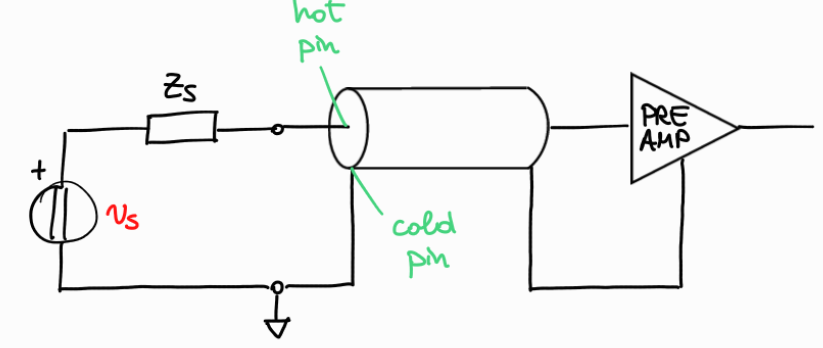
\includegraphics[width=0.90\textwidth]{Coaxial_cable_Audio_Path.png}
    \caption{Cross-section of a coaxial audio cable connecting the source (with source impedance \( Z_s \)) to the pre-amplifier. The inner conductor (hot pin) carries the signal; the outer braid (cold pin) is tied to ground and acts as an electrostatic shield, terminating the electric field lines of any external disturbance before they reach the inner conductor}
    \label{fig:coaxPath}
\end{figure}

The external braid intercepts the electric field of nearby disturbers and shunts the induced current directly to ground, preventing it from reaching the inner conductor. Magnetic disturbances (inductive coupling) are not shielded by the coaxial geometry and require balanced connections or physical separation to be attenuated.

\subsection{Distributed RC Model}

Bringing the two conductors close together to form a coaxial structure has an unavoidable consequence: the geometry creates a distributed capacitance between the inner and outer conductors. A real cable of length \( L \) is therefore modeled as a ladder network of infinitesimal elements, each comprising a series resistance \( r \cdot \mathrm{d}x \) and a shunt capacitance \( c \cdot \mathrm{d}x \), where \( r \) [\si{\ohm\per\metre}] and \( c \) [\si{\farad\per\metre}] are the per-unit-length parameters (figure \ref{fig:coaxDistrib}).

\begin{figure}[!htb]
    \centering
    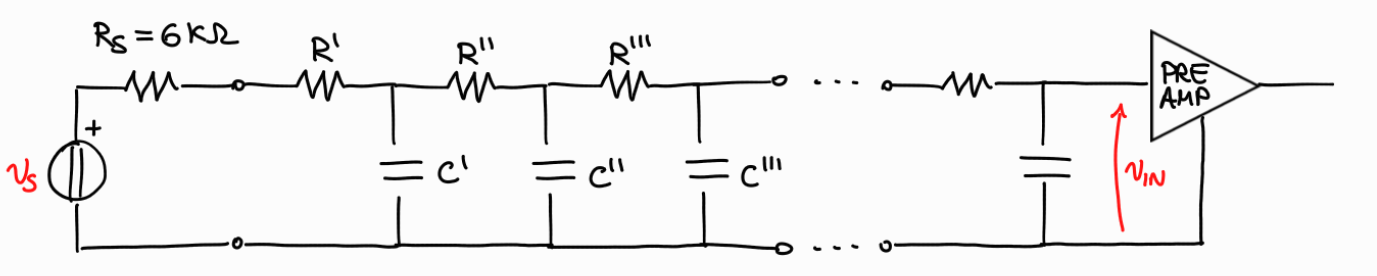
\includegraphics[width=0.90\textwidth]{Coaxial_cable_distributed_element.png}
    \caption{Distributed-element model of a coaxial cable with source impedance \( R_s = \SI{6}{\kilo\ohm} \). Each cell consists of a series resistance element \( R' \) and a shunt capacitance element \( C' \), representing the per-unit-length parameters \( r \) and \( c \) of the cable. The input voltage \( v_{IN} \) at the pre-amplifier is progressively attenuated at high frequencies as the capacitive shunt elements provide a low-impedance path to ground}
    \label{fig:coaxDistrib}
\end{figure}

For a cable of total length \( L \), the lumped equivalent parameters are:
\[
R_c = r \cdot L, \qquad C_c = c \cdot L
\]
In typical audio scenarios, \( R_c \ll R_s \) (the cable resistance is negligible compared to the source impedance), so the series resistance of the cable can be absorbed into \( R_s \). The simplified equivalent circuit then reduces to the first-order RC network of figure \ref{fig:coaxEquiv}: the source resistance \( R_s \) drives the total cable capacitance \( C_c \), forming a low-pass filter.

\begin{figure}[!htb]
    \centering
    \subfloat[Simplified equivalent circuit: \( R_s \) drives the total lumped cable capacitance \( C_c \), forming a first-order low-pass filter]{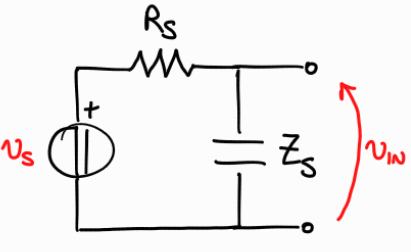
\includegraphics[width=0.40\linewidth]{coaxial_cable_equiv_scheme.png}}
    \hfill
    \subfloat[Bode magnitude plot of \( |V_{IN}/V_s| \). The pole frequency \( f_p \) marks the \SI{-3}{\decibel} point; above it the response falls at \SI{-20}{\decibel\per decade}. If \( f_p \) falls within the audio band (\SIrange{20}{20000}{\hertz}), high-frequency content is physically lost]{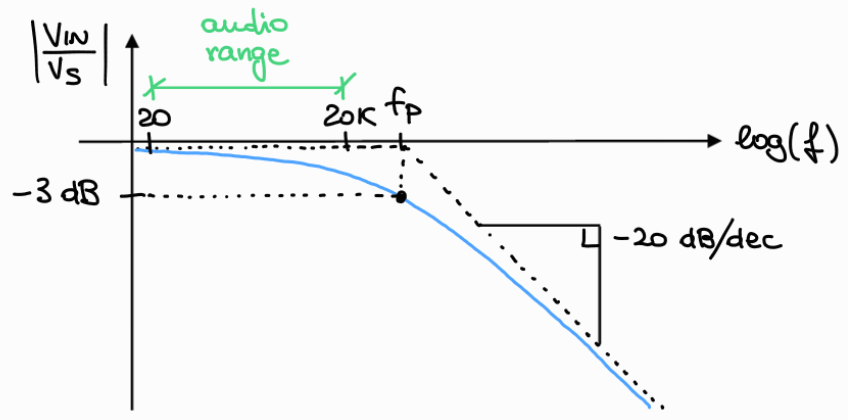
\includegraphics[width=0.52\linewidth]{Coaxial_Cable_Freq_Resp.PNG}}
    \caption{RC low-pass model of the coaxial cable (left) and its frequency response (right). The cable behaves as a first-order filter with transfer function \( V_{IN}/V_s = 1/(1 + j f/f_p) \), where \( f_p = 1/(2\pi R_s C_c) \)}
    \label{fig:coaxEquiv}
\end{figure}

The transfer function from source to amplifier input is:
\[
\frac{V_{IN}}{V_s} = \frac{Z_c}{R_s + Z_c} = \frac{1}{1 + sR_s C_c},
\qquad Z_c = \frac{1}{sC_c}
\]
This is a first-order low-pass filter with pole frequency:
\[
f_p = \frac{1}{2\pi R_s C_c}
\]

\subsection{Practical Example: Guitar Cable}

A representative real-world case is a passive electric guitar with high source impedance connected via a standard unbalanced cable.  Typical parameters are:
\[
r = \SI{80}{\milli\ohm\per\metre}, \qquad
c = \SI{100}{\pico\farad\per\metre}, \qquad
L = \SI{20}{\metre}, \qquad
R_s = \SI{6}{\kilo\ohm}
\]
The total cable resistance and capacitance are:
\[
R_c = rL = 80 \times 10^{-3} \times 20 = \SI{1.6}{\ohm} \ll R_s
\]
\[
C_c = cL = 100 \times 10^{-12} \times 20 = \SI{2}{\nano\farad}
\]
Since \( R_c \approx \SI{1.6}{\ohm} \ll R_s = \SI{6}{\kilo\ohm} \), the cable resistance is negligible and the approximation \( R_c \approx 0 \) is fully justified. The pole frequency is:
\[
f_p = \frac{1}{2\pi R_s C_c}
= \frac{1}{2\pi \times 6 000 \times 2 \times 10^{-9}}
\approx \SI{13.3}{\kilo\hertz}
\]
This result has a direct audible consequence: the \SI{-3}{\decibel} attenuation point falls at \SI{13.3}{\kilo\hertz}, well inside the top octave of the audio band (\SIrange{10}{20}{\kilo\hertz}). All frequencies above \SI{13.3}{\kilo\hertz} are progressively attenuated at \SI{-20}{\decibel\per decade}. A guitarist using a long cable and a high-impedance pickup therefore loses the upper harmonics of the instrument, perceiving the sound as darker and less detailed compared to a direct connection. The remedy is either to reduce the cable length, to use a balanced interconnection or to insert a high-impedance buffer (active DI box) at the guitar output to lower the effective source impedance seen by the cable.

\section{Open-Loop Frequency Response}
\label{sc:26}

Up to this point the operational amplifier has been treated as an ideal voltage-controlled voltage source with gain \( g \to \infty \). A more realistic model must account for the fact that the open-loop gain \( A \) is not constant but depends on frequency. Internally, every Op-Amp contains at least one dominant pole introduced deliberately by a compensation capacitor; the result is a first-order low-pass transfer function of the form:
\[
A(s) = \frac{A_0}{1 + s\tau_0}
\]
where \( A_0 \) is the DC open-loop gain and \( \tau_0 \) is the time constant associated with the dominant pole. Replacing \( s = j2\pi f \) and identifying the \SI{-3}{\decibel} corner frequency \( f_0 = 1/(2\pi\tau_0) \), equation takes the equivalent form:
\[
A(j2\pi f) = \frac{A_0}{1 + j f/f_0}
\]

\begin{figure}[!htb]
    \centering
    \subfloat[Simplified first-order model of the Op-Amp: the output is proportional to the differential input through the frequency-dependent gain \( A(s) \)]{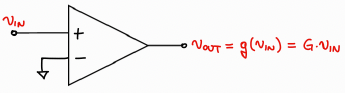
\includegraphics[width=0.45\linewidth]{OPAMP_simple_scheme.png}}
    \hfill
    \subfloat[Bode magnitude plot of the open-loop gain. The gain is flat at \( A_0 \) for \( f \ll f_0 \), rolls off at \SI{-20}{\decibel\per decade} above the pole and reaches unity (\SI{0}{\decibel}) at the unity-gain frequency \( f_u \)]{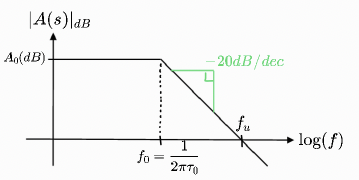
\includegraphics[width=0.45\linewidth]{OPAMP_1st_Order_Freq_Rep.png}}
    \caption{First-order open-loop model and its Bode magnitude response. The single dominant pole at \( f_0 \) determines the entire high-frequency behavior of the uncompensated amplifier}
    \label{fig:openLoopFreq}
\end{figure}

The Bode plot of figure \ref{fig:openLoopFreq} reveals immediately why an Op-Amp cannot be used in open loop in any practical audio application. On one hand, the DC gain \( A_0 \) is typically in the range of \SIrange{60}{120}{\decibel}, corresponding to linear voltage gains of \( 10^3 \) to \( 10^6 \). Even a microphone-level signal of a few millivolts would be amplified so strongly that the output would saturate against one of the supply rails almost instantaneously. On the other hand, the dominant pole \( f_0 \) is placed at an extremely low frequency, often between \SI{10}{\hertz} and a few kilohertz, depending on the device family. This means that for any frequency above \( f_0 \), which encompasses virtually the entire audible spectrum, the gain is already decreasing at \SI{-20}{\decibel\per decade} and the phase shift is growing toward \SI{-90}{\degree}. Both problems would produce a strongly nonlinear, frequency-dependent and phase-distorted amplifier, entirely incompatible with high-fidelity audio. Negative feedback, introduced in the following section, resolves both issues simultaneously.

\section{Negative Feedback}
\label{sc:27}

The idea of exploiting a large open-loop gain to obtain a well-controlled closed-loop gain was formalized by Harold Black at Bell Laboratories in 1927: deliberately build a very large forward gain and then subtract a fraction of the output back to the input. The excess gain is traded for stability, bandwidth and insensitivity to parameter variations.

\paragraph{Block diagram and the closed-loop gain} The general feedback system is described by the block diagram of figure \ref{fig:blockDiagram}, where the forward path has transfer function \( A(s) \) (the Op-Amp) and the feedback path has transfer function \( F(s) \) (typically a passive network). Three signals are defined: the input \( S_{in} \), the feedback signal \( S_f = F(s) S_{out} \) and the error signal \( \varepsilon = S_{in} - S_f \). The output satisfies \( S_{out} = A(s) \varepsilon \), so:
\[
S_{out} = A(s)\bigl[S_{in} - F(s) S_{out}\bigr]
\quad\Longrightarrow\quad
S_{out}\bigl[1 + A(s)F(s)\bigr] = A(s) S_{in}
\]

\begin{figure}[!htb]
    \centering
    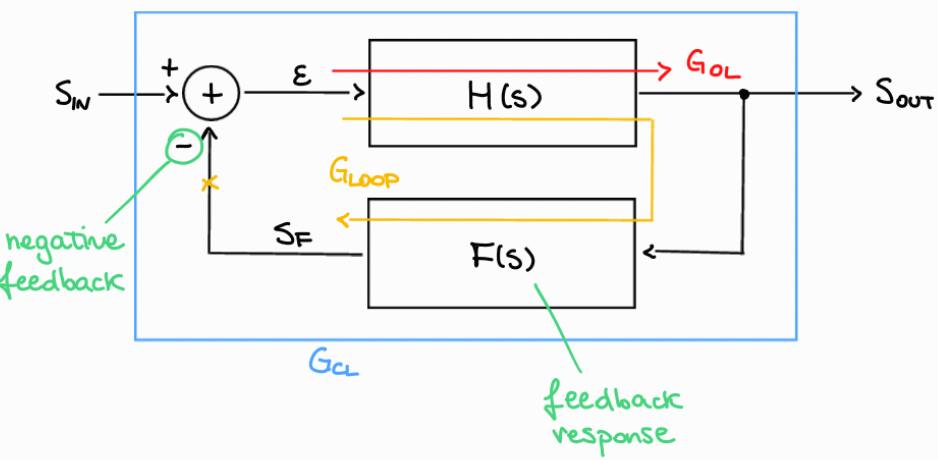
\includegraphics[width=0.90\textwidth]{OPAMP_Block_Diagram.png}
    \caption{Feedback block diagram. The forward amplifier \( A(s) \) is driven by the error signal \( \varepsilon = S_{in} - S_f \); the feedback network \( F(s) \) returns a fraction of the output to the summing junction}
    \label{fig:blockDiagram}
\end{figure}

Defining the loop gain \( G_{LOOP}(s) = A(s)F(s) \), the closed-loop gain is:
\[
G_{CL}(s) = \frac{S_{out}}{S_{in}} = \frac{A(s)}{1 + A(s)F(s)} = \frac{A(s)}{1 + G_{LOOP}(s)}
\]
For voltage signals, \( S_{in} = v_{in} \), \( S_{out} = v_{out} \) and it becomes the standard closed-loop voltage gain of the Op-Amp.

\subsection{Sensitivity and Stability}

A primary motivation for negative feedback is the dramatic reduction in sensitivity of the closed-loop gain to variations in \( A(s) \). Without feedback, the system gain equals \( A(s) \) directly, so a relative variation \( dA/A \) produces an identical relative variation \( dG/G = dA/A \) in the output. This is unacceptable in practice because \( A(s) \) depends strongly on temperature, supply voltage and fabrication spread. Differentiating with respect to \( A \) the equation that defines \( G_{CL}(s) \) yields:
\[
\frac{dG_{CL}}{dA} = \frac{(1 + AF) - AF}{(1 + AF)^2} = \frac{1}{(1 + AF)^2}
\]
Converting to relative quantities:
\[
\frac{dG_{CL}}{G_{CL}} = \frac{1}{G_{CL}}\cdot\frac{dG_{CL}}{dA}\cdot dA
= \frac{1+AF}{A}\cdot\frac{1}{(1+AF)^2}\cdot dA
= \frac{1}{1 + A(s)F(s)}\cdot\frac{dA}{A}
\]
This result shows that the relative change in the closed-loop gain is suppressed by the factor \( 1/(1+AF) \) relative to the open-loop variation. For example, with \( G_{LOOP} = AF = 100 \), a \SI{10}{\percent} drift in \( A \) produces only a \SI{0.1}{\percent} drift in \( G_{CL} \): the feedback reduces the sensitivity by three orders of magnitude.

\subsection{Attenuation Feedback and the Non-Inverting Amplifier}

When \( AF \gg 1 \), the closed-loop gain simplifies to:
\[
G_{CL} = \frac{A}{1 + AF} \approx \frac{A}{AF} = \frac{1}{F}
\]
and is set almost entirely by the feedback network \( F \), independent of \( A \). In audio pre-amplifiers the feedback network is almost universally a resistive voltage divider, which provides a frequency-independent attenuation \( F < 1 \). The non-inverting configuration shown in figure \ref{fig:attenFB} connects the output through a resistive divider \( R_1, R_2 \) to the inverting input.

\begin{figure}[!htb]
    \centering
    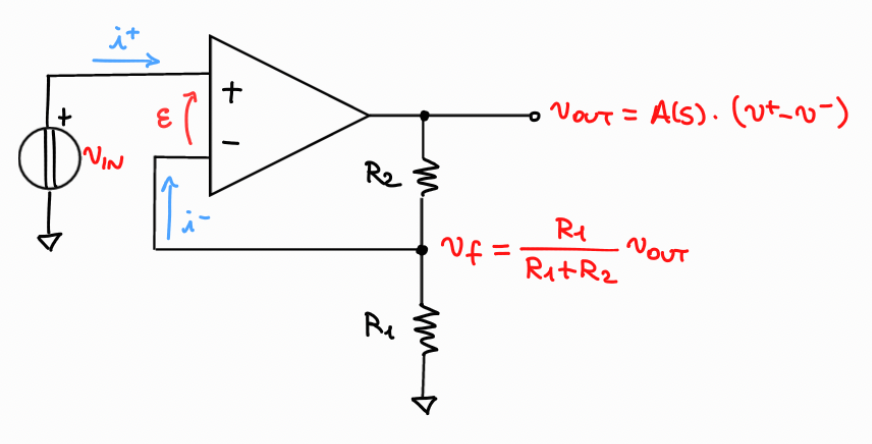
\includegraphics[width=0.90\textwidth]{Attenuation_FB_Response.png}
    \caption{Non-inverting amplifier with resistive feedback. The divider \( R_1, R_2 \) sets the feedback factor \( F = R_1/(R_1+R_2) \); the closed-loop gain is \( G_{CL} = 1 + R_2/R_1 \) when the loop gain is large}
    \label{fig:attenFB}
\end{figure}

The feedback voltage at the inverting input is:
\[
v^{-} = v_{out} \frac{R_1}{R_1 + R_2}
\quad\Longrightarrow\quad F = \frac{R_1}{R_1 + R_2}
\]
Substituting into the closed-loop gain for \( AF \gg 1 \):
\[
G_{CL} \approx \frac{1}{F} = \frac{R_1 + R_2}{R_1} = 1 + \frac{R_2}{R_1}
\]
This is one of the most important results in analog circuit design. The gain is set by the ratio of two resistors, which can be matched and track each other with temperature to high accuracy (typical temperature coefficient \( \alpha_T \approx \SI{10}{\ppm\per\kelvin} \)), making the amplifier gain essentially temperature-invariant. The condition \( G_{CL} \geq 1 \) is automatically satisfied, confirming that the non-inverting topology can only amplify, never attenuate.

\paragraph{Virtual short circuit} Since the output voltage is finite and \( A_0 \) is very large, the error signal must be vanishingly small: \( \varepsilon = v_{out}/A \approx 0 \). This forces the two input terminals to be virtually at the same potential, \( v^{+} \approx v^{-} \), even though they are not galvanically connected. Combined with the infinite input impedance assumption (\( i^{+} = i^{-} = 0 \)), this virtual short circuit is the fundamental working hypothesis for analyzing any Op-Amp circuit operating well within its linear range.

\section{Gain-Bandwidth Product and Closed-Loop Bandwidth}
\label{sc:28}

\subsection{Unity-Gain Frequency}

Above the dominant pole frequency \( f_0 \), the open-loop gain rolls off at \SI{-20}{\decibel\per decade}, yet the product \( |A(j2\pi f)|\cdot f \) remains nearly constant in that region. For \( f \gg f_0 \):
\[
|A(j2\pi f)| \approx \frac{A_0 f_0}{f}
\]
The unity-gain frequency \( f_u \) is defined as the frequency at which the open-loop magnitude equals one (\SI{0}{\decibel}). Setting \( |A(j2\pi f_u)| = 1 \) and using the approximation \( A_0^2 \gg 1 \):
\[
\frac{A_0}{|1 + j f_u/f_0|} = 1
\quad\Longrightarrow\quad
A_0^2 = 1 + \left(\frac{f_u}{f_0}\right)^2 \approx \left(\frac{f_u}{f_0}\right)^2
\quad\Longrightarrow\quad
f_u = A_0 f_0
\]
The quantity \( A_0 f_0 \) is therefore equal to \( f_u \) and defines the Gain-Bandwidth Product (GBWP):
\[
\mathrm{GBWP} = A_0 f_0 = f_u
\]
The GBWP is listed in every Op-Amp datasheet as a figure of merit: a higher GBWP enables either a larger closed-loop gain or a wider bandwidth for the same device.

\subsection{The Closed-Loop Bandwidth and the Gain-Bandwidth Trade-off}

When negative feedback is applied, the closed-loop gain is constant at \( G_{CL} = 1/F \) for all frequencies where \( G_{LOOP} \gg 1 \), but the loop gain itself is frequency-dependent because \( A(s) \) rolls off. Figure \ref{fig:feedbackFreqResp} shows the relationship between the open-loop gain curve, the closed-loop gain level and the loop gain on a Bode diagram.

\begin{figure}[!htb]
    \centering
    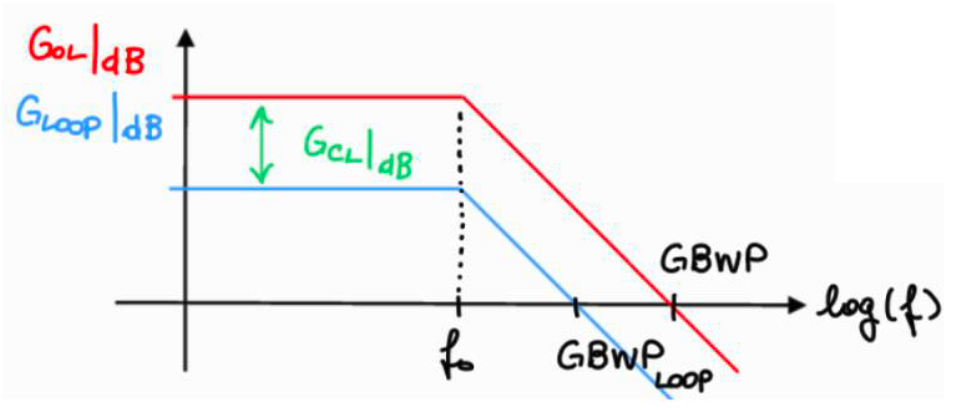
\includegraphics[width=0.90\textwidth]{Freq_Resp_FeedBack_OPAMP.png}
    \caption{Bode magnitude diagram of the feedback amplifier. The open-loop gain \( A(f) \) (upper curve) intersects the closed-loop gain level \( G_{CL} = 1/F \) (horizontal line) at the closed-loop \SI{-3}{\decibel} frequency \( f_{0,CL} \). The loop gain \( G_{LOOP}|_{dB} = A|_{dB} - G_{CL}|_{dB} \) is the vertical distance between the two curves and reaches zero at the same crossover point}
    \label{fig:feedbackFreqResp}
\end{figure}

For frequencies well above \( f_0 \), the loop gain can be written as:
\[
G_{LOOP}(f) = A(f)\cdot F = \frac{A_0 f_0}{f}\cdot F = \frac{A_0 f_0}{G_{CL}\cdot f} = \frac{\mathrm{GBWP}}{G_{CL}\cdot f}
\]
The practical working range of the amplifier is the frequency interval where the feedback remains effective, conventionally defined by \( G_{LOOP}(f) \geq G_{LOOP}^{min} = 10 \). Applying this condition:
\[
\frac{\mathrm{GBWP}}{G_{CL}\cdot f} \geq 10
\quad\Longrightarrow\quad
f_{max} \leq \frac{\mathrm{GBWP}}{10\cdot G_{CL}}
\]
The new \SI{-3}{\decibel} closed-loop bandwidth (the frequency at which the loop gain crosses unity) is:
\[
f_{0,CL} = \frac{A_0}{G_{CL}}\cdot f_0 = \frac{\mathrm{GBWP}}{G_{CL}}
\]
This equation encapsulates the fundamental trade-off of any single-pole feedback amplifier: increasing the closed-loop gain \( G_{CL} \) narrows the bandwidth proportionally, while the product \( G_{CL}\cdot f_{0,CL} = \mathrm{GBWP} \) remains constant.

\paragraph{Audio design example} A professional-grade Op-Amp with \( \mathrm{GBWP} = \SI{20}{\mega\hertz} \) must cover the full audio band up to \SI{20}{\kilo\hertz}. Requiring \( G_{LOOP}(f_{max}) \geq 10 \) at \( f_{max} = \SI{20}{\kilo\hertz} \), the maximum closed-loop gain that still preserves a flat response across the audio band is:
\[
G_{CL}^{max} = \frac{\mathrm{GBWP}}{10\cdot f_{max}} = \frac{20\times10^6}{10\times 20\times10^3} = 100
\]
Equivalently, in \si{\decibel}: \( G_{CL}^{max} = \SI{40}{\decibel} \). A designer requiring higher gain must either select a device with a larger GBWP or accept a reduced usable bandwidth. The following values summarize the required GBWP for three representative gain settings:
\[
\begin{cases}
    G_{CL} = 1   & \Rightarrow\; \mathrm{GBWP} \geq 10 \times \SI{20}{\kilo\hertz} = \SI{200}{\kilo\hertz}\\
    G_{CL} = 10  & \Rightarrow\; \mathrm{GBWP} \geq 10 \times \SI{20}{\kilo\hertz} \times 10 = \SI{2}{\mega\hertz}\\
    G_{CL} = 100 & \Rightarrow\; \mathrm{GBWP} \geq 10 \times \SI{20}{\kilo\hertz} \times 100 = \SI{20}{\mega\hertz}
\end{cases}
\]

\section{Slew Rate and Full-Power Bandwidth}
\label{sc:29}

The GBWP analysis assumes small-signal conditions, where the amplifier operates in its linear regime. A separate, independent limitation governs large-signal behavior: the maximum rate of change of the output voltage per unit time. This physical constraint, known as the slew rate (SR), arises from the finite current available to charge the internal compensation capacitor:
\[
\left.\frac{dv_{out}}{dt}\right|_{max} = \mathrm{SR} \qquad [\si{\volt\per\micro\second}]
\]

\paragraph{Full-Power Bandwidth}
Consider a sinusoidal output at the maximum permissible amplitude \( \hat{V} = V_{out}^{max} \):
\[
v_{out}(t) = V_{out}^{max}\sin(\omega t)
\quad\Longrightarrow\quad
\frac{dv_{out}}{dt} = V_{out}^{max} \omega\cos(\omega t)
\]
The instantaneous rate of change is maximized at the zero crossing of the sinusoid, where it reaches \( V_{out}^{max} \omega \). For the amplifier to reproduce this waveform faithfully, this peak slope must not exceed the slew rate:
\[
V_{out}^{max} \omega_{max} \leq \mathrm{SR}
\quad\Longrightarrow\quad
\omega_{max} = \frac{\mathrm{SR}}{V_{out}^{max}}
\]
The corresponding frequency defines the Full-Power Bandwidth (FPBW):
\[
f_{FPBW} = \frac{\mathrm{SR}}{2\pi V_{out}^{max}}
\]
The FPBW is the highest frequency at which the amplifier can reproduce a sinusoidal output at full rated amplitude without slew-rate-induced waveform degradation. In most Op-Amps it lies below the bandwidth predicted by the GBWP; of the two limits, the binding constraint for a given operating condition is always the lower one.

\subsection{Slew-Rate-Induced Distortion}

When the operating frequency or the output amplitude exceeds the FPBW limit, the output no longer clips horizontally as in conventional signal clipping but instead follows the maximum-slope ramp imposed by the slew rate. The consequence is that a sinusoidal input produces a triangular output waveform, as illustrated in figure \ref{fig:slewRate}. A triangular waveform at the fundamental frequency contains substantial odd-order harmonic content (third, fifth, seventh\ldots), which rises abruptly once the slew-rate limit is exceeded. This produces a sharp increase in Total Harmonic Distortion (THD) at high frequencies and high output levels, an effect that manifests as harshness or hardness in audio reproduction and that is fundamentally different from the gentler onset of small-signal bandwidth roll-off. The equation that defines \( f_{FPBW} \) is therefore the relevant specification when selecting an Op-Amp for high-power, high-frequency audio applications such as active loudspeaker crossovers or headphone amplifiers.

\begin{figure}[!htb]
    \centering
    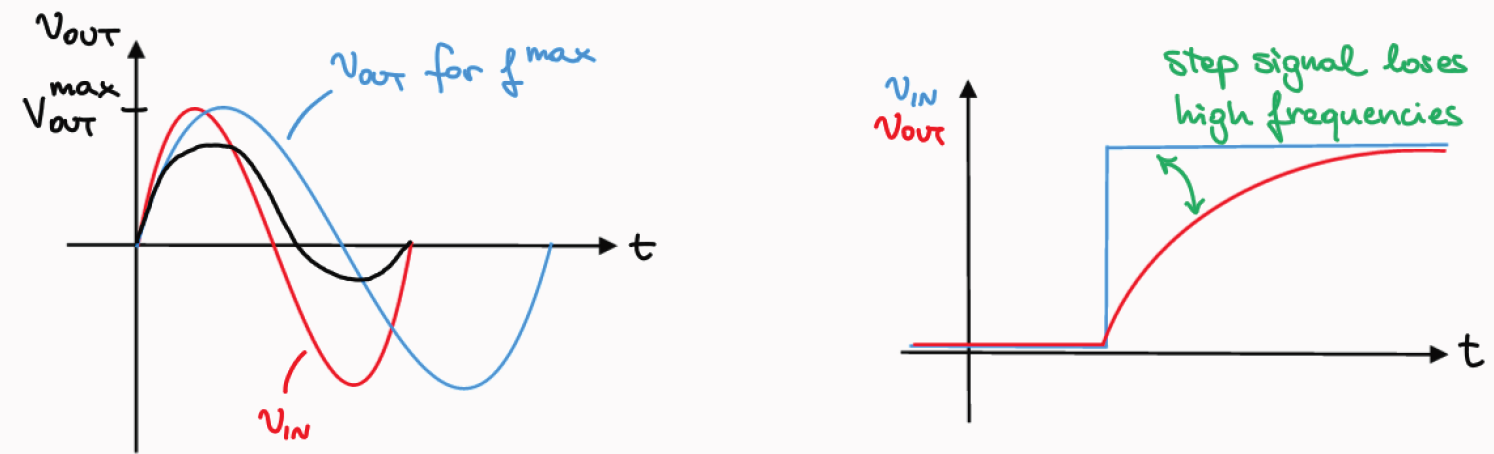
\includegraphics[width=0.90\textwidth]{Slew_Rate_Illustration.png}
    \caption{Effect of slew-rate limiting on a sinusoidal signal. Above the FPBW limit, the output (dashed) can no longer follow the rising and falling edges of the input (solid) and degrades into a triangular approximation; the resulting spectrum contains large odd-order harmonics that sharply increase the Total Harmonic Distortion (THD) at high frequencies and high output levels}
    \label{fig:slewRate}
\end{figure}

\section{The Inverting Configuration}
\label{sc:30}

The non-inverting amplifier analysed in section \ref{sc:26} produces an output in phase with the input and imposes a closed-loop gain \( G_{CL} = 1 + R_2/R_1 \geq 1 \). An equally important topology is the inverting configuration, shown in figure \ref{fig:invertConfig}, where the signal is applied to the inverting input through \( R_1 \) and the feedback resistor \( R_2 \) connects the output back to the same node.
The non-inverting input is tied to ground.

\begin{figure}[!htb]
    \centering
    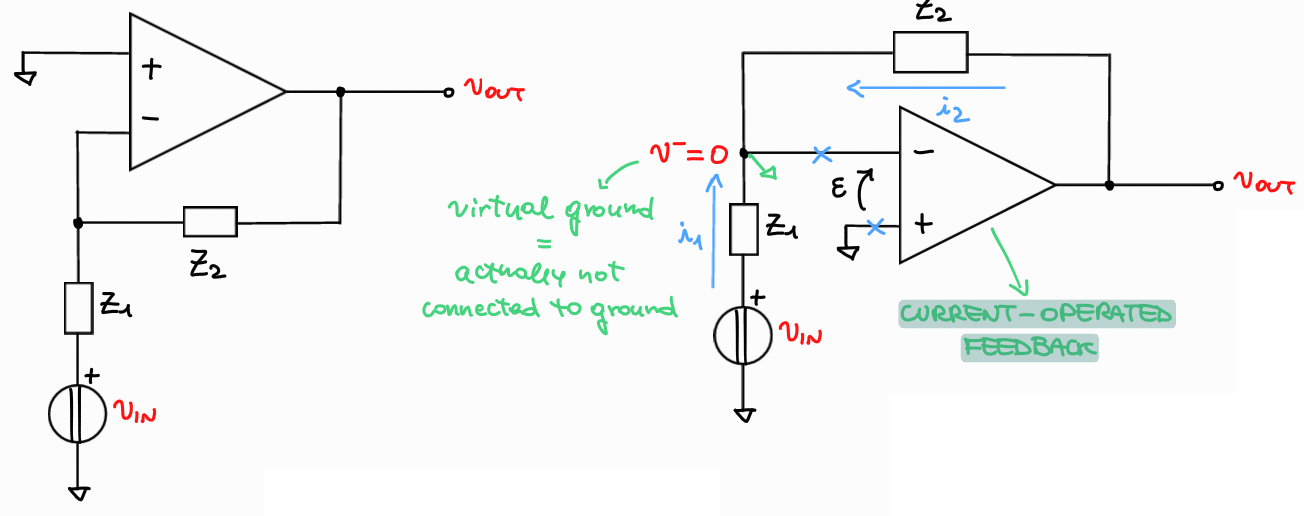
\includegraphics[width=0.90\textwidth]{OPAMP_Invert_Config_Generalized.png}
    \caption{Inverting amplifier. The source is applied to the \( v^{-} \) pin through \( R_1 \); the feedback resistor \( R_2 \) connects the output back to the same node. The non-inverting input is held at ground, making the inverting node a virtual ground under ideal conditions}
    \label{fig:invertConfig}
\end{figure}

The transfer function is derived in three steps, starting from the two ideal Op-Amp assumptions: the error signal is vanishingly small (\( \varepsilon \approx 0 \), virtual short circuit), and no current flows into either input terminal (\( i^{+} = i^{-} = 0 \)).

\paragraph{Step 1: current through \( R_1 \)} Since \( v^{+} = 0 \) and the virtual short circuit forces \( v^{-} = v^{+} = 0 \), the inverting node is a virtual ground.
The current flowing from the source into \( R_1 \) is:
\[
i_1 = \frac{v_{in} - v^{-}}{R_1} = \frac{v_{in}}{R_1}
\]

\paragraph{Step 2: current through \( R_2 \)} The current leaving the inverting node through \( R_2 \) toward the output is:
\[
i_2 = \frac{v^{-} - v_{out}}{R_2} = \frac{-v_{out}}{R_2}
\]

\paragraph{Step 3: KCL at the inverting node} Because no current enters the inverting input (\( i^{-} = 0 \)), all of \( i_1 \) must flow through \( R_2 \):
\[
i_1 = i_2
\quad\Longrightarrow\quad
\frac{v_{in}}{R_1} = \frac{-v_{out}}{R_2}
\quad\Longrightarrow\quad
\frac{v_{out}}{v_{in}} = -\frac{R_2}{R_1}
\]
The closed-loop voltage gain of the inverting amplifier is therefore:
\[
G_{CL}^{INV} = -\frac{R_2}{R_1}
\]
The magnitude \( |G_{CL}^{INV}| = R_2/R_1 \) can be set freely to any value above or below unity by choosing the resistor ratio, in contrast to the non-inverting topology which is bounded below by 1. The negative sign indicates a \SI{180}{\degree} phase inversion: the output is a sign-inverted, scaled replica of the input. This property is exploited in summing amplifiers, active filters, and differential stages wherever polarity reversal is either desired or algebraically required.

\section{Gain Control and Signal Level Control}
\label{sc:210}

In the design of audio systems a fundamental distinction must be maintained between two operations that are superficially similar but physically different.

\paragraph{Gain control} modifies the amplification factor of a stage, for instance by changing the resistor ratio \( R_2/R_1 \) of the feedback network. The intrinsic transfer function of the stage is altered.

\paragraph{Signal level control} adjusts the amplitude of the signal at a given point in the chain, typically by attenuating the voltage through a passive voltage divider, without altering the internal gain of any amplifying stage. A potentiometer placed before or after an amplifier stage performs signal level control: the stage gain is unchanged; only the signal amplitude entering or leaving the stage is varied. The distinction has a direct consequence for audio quality. Non-linear distortion is generated inside the amplifying stages, so only controls placed before those stages can modify how much distortion is produced. A level control placed after all non-linear elements can reduce loudness but cannot undo the harmonic content already generated. This point is illustrated concretely in the case study of section \ref{sc:212}.

\section{Nominal Signal Levels and Audio References}
\label{sc:211}

Audio signals fluctuate continuously in amplitude; using the instantaneous peak value to characterize signal strength is impractical because the peak depends on transient content and does not correlate well with perceived loudness or average power. The standard descriptor is instead the Nominal Signal Level, defined in terms of the RMS voltage.
Recalling the fundamental relations:
\[
P(t) = \frac{v^2(t)}{R},
\qquad
\overline{P} = \frac{1}{R}\cdot\frac{1}{T}\int_0^T v^2(t) dt,
\qquad
v_{RMS} = \sqrt{\frac{1}{T}\int_0^T v^2(t) dt}
\]
the RMS voltage is the constant DC voltage that would dissipate the same average power \( \overline{P} \) in the same resistance \( R \), and therefore provides a physically meaningful and time-stable descriptor of signal level. Two logarithmic scales are used in professional audio.
The dBV scale references the signal to \SI{1}{\volt} RMS:
\[
\mathrm{dBV} = 20\log_{10} \left(\frac{V_{sig}}{\SI{1}{\volt}}\right)
\]
The dBu scale references the signal to the voltage that delivers \SI{1}{\milli\watt} into the historical \SI{600}{\ohm} telephone-system load:
\[
V_{ref} = \sqrt{10^{-3}\times 600} \approx \SI{0.7746}{\volt},
\qquad
\mathrm{dBu} = 20\log_{10} \left(\frac{V_{sig}}{\SI{0.7746}{\volt}}\right)
\]
The dBu scale is the standard in professional audio interfaces and mixing consoles, and is invariant to load impedance because the \SI{600}{\ohm} reference is historical rather than an actual termination requirement in modern equipment.

\subsection{Dynamic Range and the ADC}

The pre-amplification stage must raise the signal to a level that occupies the intended portion of the converter input dynamic range (IDR), as shown in figure \ref{fig:adcChain}.

\begin{figure}[!htb]
    \centering
    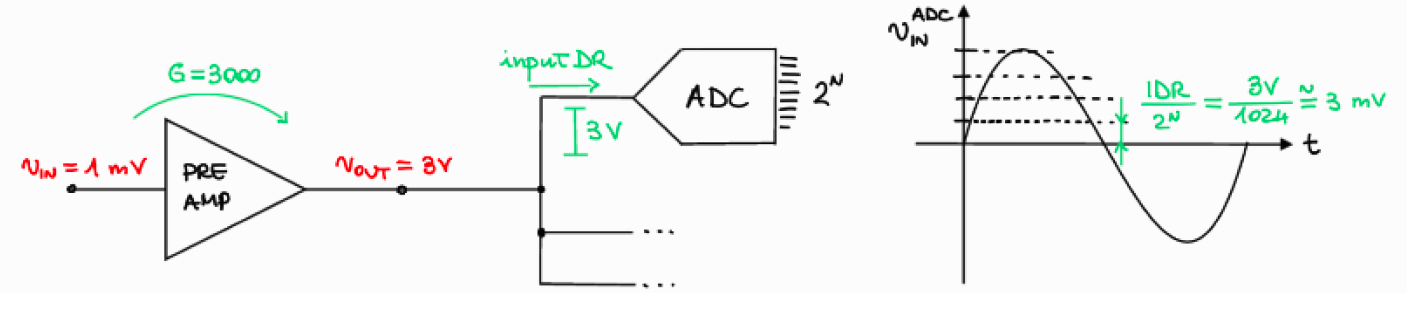
\includegraphics[width=0.65\textwidth]{Dynamic_Range_with_ADC.png}
    \caption{Pre-amplification stage feeding an analog-to-digital converter. The pre-amp gain must place the nominal output level within the IDR, with sufficient headroom below the full-scale clipping level and sufficient margin above the quantization noise floor}
    \label{fig:adcChain}
\end{figure}

In a converter with \( N \)-bit resolution and full-scale amplitude \( V_{FS} \), the voltage step corresponding to the least significant bit is:
\[
V_{LSB} = \frac{V_{FS}}{2^N}
\]
For a 24-bit converter with \( V_{FS} = \SI{3}{\volt} \), this gives \( V_{LSB} \approx \SI{0.18}{\micro\volt} \). This value is so small that the analog front-end noise and the accuracy of the preamplifier gain become the binding constraints on overall system resolution, not the converter word length itself. The required precision of gain setting therefore rises with the word length of the converter, motivating the use of temperature-stable resistor networks and feedback-based gain stages rather than open-loop configurations.

\section{Sensitivity}
\label{sc:213}

The sensitivity \( S \) of a gain stage is the input voltage required to produce the desired nominal output level:
\[
S = \frac{V_{out}^{nom}}{G}
\]
A counterintuitive but practically important consequence is that increasing the gain \( G \) reduces the numerical value of \( S \): a higher-gain stage requires a smaller input signal to reach the same output level and is therefore more sensitive to weak inputs and to noise. In power amplifier datasheets, a notable example being the Crown series used widely in professional live sound, the sensitivity specification is listed instead of the gain. The reason is that the end-user workflow is to set the input trim until a target output power is reached, rather than to work from a gain figure. For example, a power amplifier with a nominal output of \SI{28}{\volt} and a voltage gain of 28 has a sensitivity of \( S = \SI{1}{\volt} \approx \SI{2.2}{\decibel u} \); if the gain is raised to 100, the sensitivity decreases to \( S = \SI{0.28}{\volt} \approx \SI{-9.1}{\decibel u} \), meaning the amplifier now reaches full output with a much weaker source signal and is correspondingly more susceptible to hum and noise at the input.

\section{Potentiometers}
\label{sc:214}

A potentiometer is a three-terminal resistive element with a movable wiper. Denoting the wiper position as \( x \in [0, L] \) for a slide type and the total resistance as \( R_{POT} \), the two partial resistances satisfy:
\[
R_{1,3} = \frac{x}{L} R_{POT},
\qquad
R_{2,3} = \frac{L-x}{L} R_{POT},
\qquad
R_{1,3} + R_{2,3} = R_{POT}
\]
regardless of wiper position.
Connected as a voltage divider, the wiper output varies continuously from \SI{0}{\volt} to \( V_{in} \), providing a continuously variable attenuation.

\begin{figure}[!htb]
    \centering
    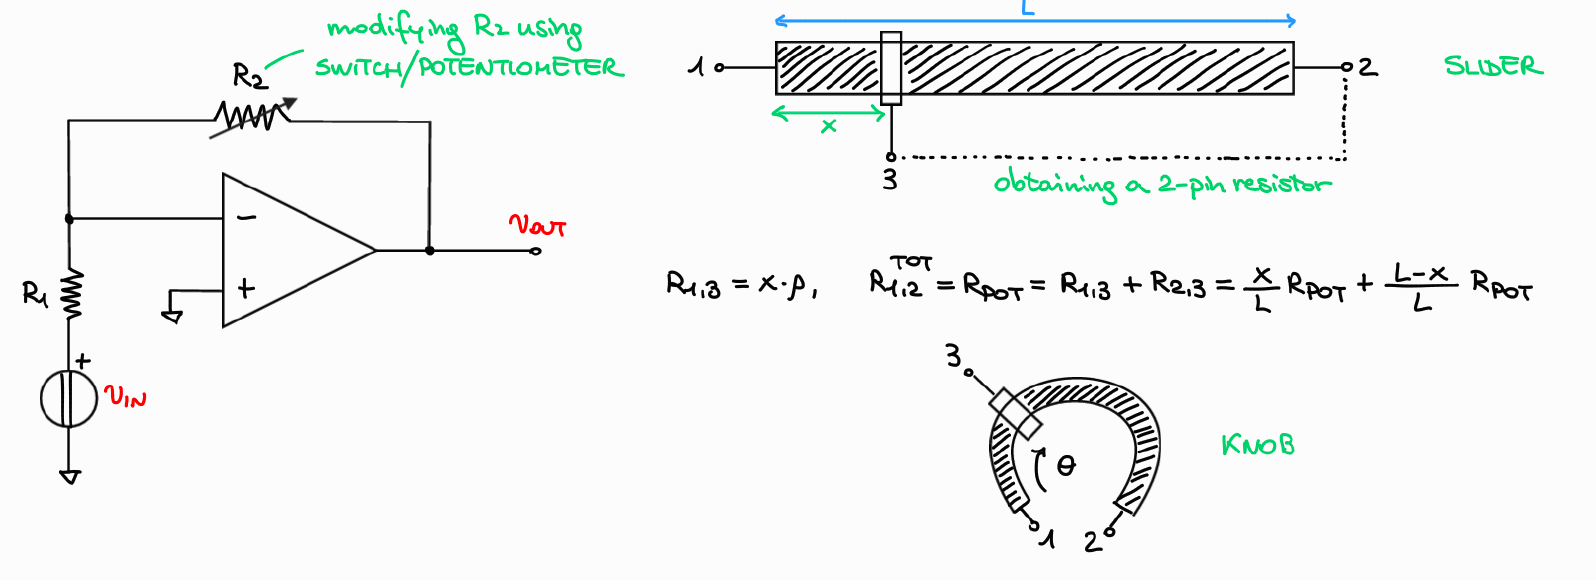
\includegraphics[width=0.90\textwidth]{Potentiometers.png}
    \caption{Potentiometer connected for gain control in a non-inverting Op-Amp stage (left) and schematic of the resistive element with the wiper dividing it into segments \( R_{1,3} \) and \( R_{2,3} \) (right). In a dual-gang potentiometer two resistive bars are mechanically coupled to the same shaft, ensuring simultaneous and matched adjustment of two channels}
    \label{fig:pots}
\end{figure}

Potentiometers are manufactured in three principal mechanical forms: rotary (single or dual-gang for stereo), slide (faders in mixing consoles), and trimmer (miniature screwdriver-adjusted elements for factory calibration).

\subsection{The Problem of Linear Potentiometers in Audio}

A linear potentiometer provides a resistance proportional to wiper displacement. Because human loudness perception is approximately logarithmic, a perceived doubling of loudness corresponds to a \SI{10}{\decibel} increase in power, not a doubling of it, a linear resistance taper maps physical rotation highly non-uniformly to perceived volume. In practice, the first half of the travel changes the level by only a few decibels while the upper half covers most of the audible dynamic range, making fine low-level adjustment impossible and high-level adjustment dangerously abrupt.

\subsection{Logarithmic Potentiometers: Mathematical Derivation}

To produce perceptually uniform control, the resistance must vary exponentially with wiper position.
The required law is:
\[
R_{1,3}(\theta) = R_{POT}\times 10^{m \left(\frac{\theta}{\theta_{max}} - 1\right)}
\]
where \( \theta \) is the rotation angle, \( \theta_{max} \) the full travel, and \( m \) a curvature parameter (typically \( m = 2 \) or \( m = 3 \)).
The reason this law achieves perceptually uniform control follows directly: the signal attenuation in decibels is:
\[
L_{dB} = 20\log_{10} \left(\frac{R_{1,3}}{R_{POT}}\right)
= 20\log_{10} \left(10^{m(\theta/\theta_{max}-1)}\right)
= 20 m \left(\frac{\theta}{\theta_{max}} - 1\right)
\]
This is a linear function of the rotation angle \( \theta \), so equal increments of knob rotation produce equal increments of level in decibels, which is precisely the scale on which the auditory system integrates loudness.

\begin{figure}[!htb]
    \centering
    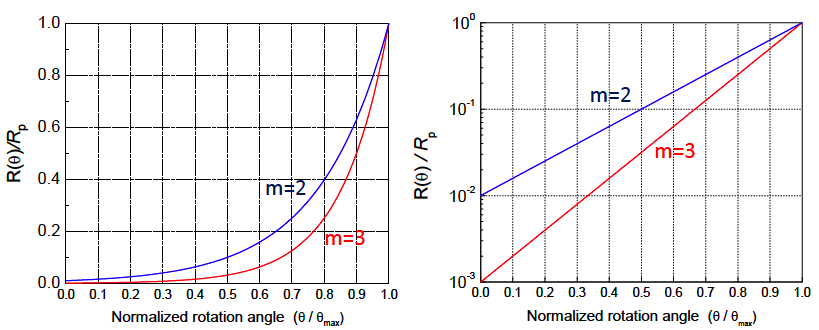
\includegraphics[width=0.90\textwidth]{Logarithmic_Pot.png}
    \caption{Normalized resistance \( R_{1,3}/R_{POT} \) as a function of normalized rotation angle for logarithmic potentiometers with \( m = 2 \) and \( m = 3 \). Left: linear vertical scale, showing the highly skewed shape. Right: logarithmic vertical scale, confirming that the resistance changes as a straight line in dB per unit angle, producing perceptually uniform loudness variation}
    \label{fig:logpot}
\end{figure}

\subsection{Digital Potentiometers}

Modern signal processing systems increasingly replace mechanical potentiometers with digital potentiometers: integrated circuits consisting of a resistor ladder and a bank of MOS switches. An \( N \)-bit digital word selects one tap of the ladder, yielding \( 2^N \) discrete resistance steps between the end terminals and the wiper output. The principal advantages over mechanical devices are the ability to change settings instantaneously under microcontroller command, to store and recall preset positions in non-volatile memory, and to eliminate contact noise and mechanical wear. The main disadvantage is the generation of switching artifacts during rapid level changes. When the wiper steps from one tap to the next, the discrete voltage discontinuity at the output is heard as a click or zipper noise. In a mechanical potentiometer the physical hand motion enforces a continuous trajectory through all intermediate resistance values, so no such discontinuity arises. Advanced digital potentiometer designs mitigate this by incorporating zero-crossing detectors that delay the tap switch until the signal passes through zero, reducing but not fully eliminating the switching glitch. The choice between digital and mechanical potentiometers therefore involves a trade-off between programmability and analog signal purity.

\section{Audio Applications: Mixing Consoles and Guitar Amplifiers}
\label{sc:212}

\subsection{Mixing Consoles}

A professional mixing console makes the distinction between gain control and signal level control immediately visible in the physical layout of each channel strip. At the top of the strip, the trim or gain knob adjusts the closed-loop gain of the microphone preamplifier stage: it modifies the feedback resistor ratio and therefore changes the true amplification factor. Setting the trim correctly, so that the nominal input signal occupies the intended operating range of the channel, is the first and most critical adjustment because every subsequent noise and distortion specification depends on the signal-to-noise ratio established at this stage. The faders at the bottom of the strip are slide potentiometers acting as signal level controls. They attenuate the amplified signal before it is routed to the summing bus, without affecting the preamplifier gain. Notably, the \SI{0}{\decibel} mark on a fader is not placed at the maximum mechanical travel but slightly below it, typically at around \SI{75}{\percent} of the physical stroke. This calibration provides headroom: the engineer can push the fader above the nominal \SI{0}{\decibel} position by a few decibels to compensate for unexpectedly quiet sources during a live performance without having to readjust the gain structure.

\subsection{Case Study: Marshall JCM 800}
\label{sc:JCM800}

The Marshall JCM 800 guitar amplifier is a canonical example of how the position of a level control in the signal chain determines its sonic effect, even when both controls present on the front panel are electrically voltage dividers (figure \ref{fig:marshall}).

\begin{figure}[!htb]
    \centering
    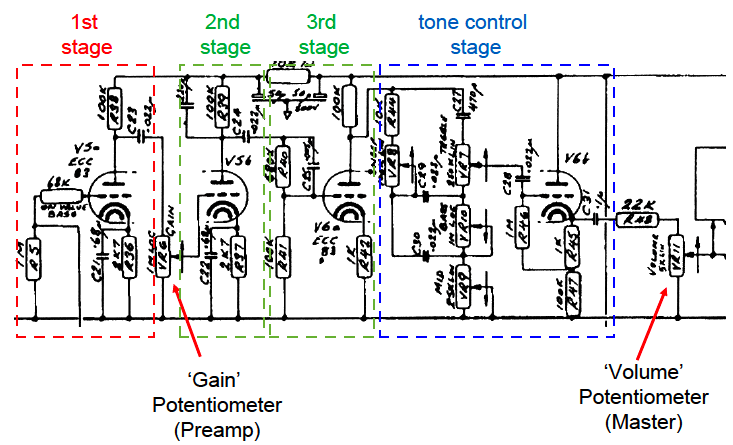
\includegraphics[width=0.90\textwidth]{Marshall_JCM_800.png}
    \caption{Signal chain of the Marshall JCM 800. The Gain potentiometer (red) is a voltage divider between the first and second preamplifier stages; the Volume potentiometer (blue) is a voltage divider at the input of the output stage. Both are signal level controls, but their positions relative to the non-linear tube stages produce entirely different sonic effects}
    \label{fig:marshall}
\end{figure}

\paragraph{Gain potentiometer} Placed between the first and second preamplifier tube stages, this control attenuates the output of the first stage before it enters the second. Because the second stage is designed to saturate at high signal levels and generate the characteristic valve overdrive, advancing the Gain pot drives the second stage harder into its non-linear region, increasing THD and shaping the harmonic content. The Gain pot sits before the distorting element, so it directly controls how much distortion is generated.

\paragraph{Volume potentiometer} Placed at the input of the power amplifier output stage, after all the preamplifier stages that produce distortion, this control scales the already-distorted signal before it is amplified to loudspeaker power. Its sole effect on timbre is a uniform level change: no new distortion is introduced and no existing harmonic content is removed. The practical consequence is the well-known technique of setting the Gain control high to obtain a heavily distorted preamp sound, then reducing the master Volume to bring the acoustic output to a comfortable level while preserving the distortion character. Both potentiometers are signal level controls; their entirely different sonic roles arise solely from their position relative to the non-linear elements in the chain.

\section{Topics Covered in A.Y. 2024/2025 that could be Useful}

\subsection{The Voltage Buffer}

A special and practically important case arises when the feedback factor is set to unity, \( F = 1 \), obtained either by setting \( R_1 \to \infty \) (open-circuiting the lower resistor) or by connecting the output directly to the inverting input (\( R_2 = 0 \)). In both cases:
\[
G_{CL} \approx \frac{1}{F} = 1,
\qquad v^{+} = v^{-} = v_{out} = v_{in}
\]

\begin{figure}[!htb]
    \centering
    \subfloat[Buffer with \( R_1 \to \infty \): no lower resistor; the output feeds the inverting input directly through the upper resistor, which carries no current]{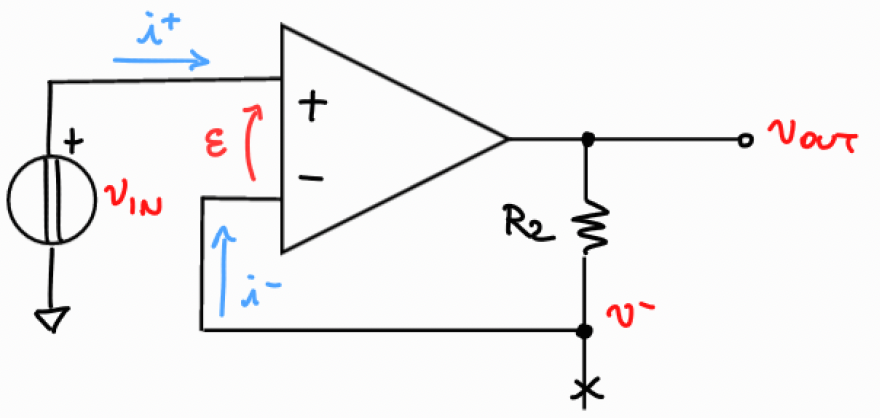
\includegraphics[width=0.44\linewidth]{OPAMP_Buffer_Mode.png}}
    \hfill
    \subfloat[Buffer with \( R_2 = 0 \): the output wire connects directly to the inverting input, yielding unity gain with minimal component count]{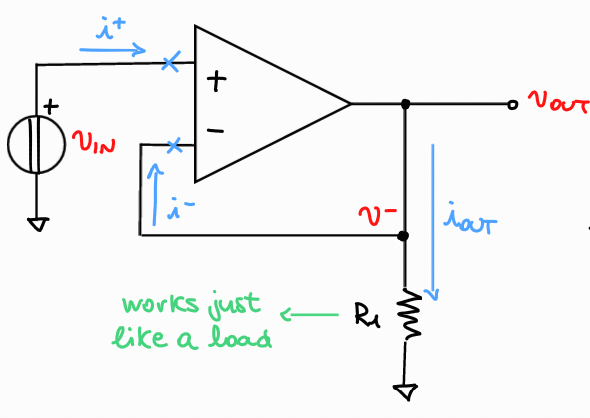
\includegraphics[width=0.44\linewidth]{OPAMP_Buffer_Mode_2nd_config.png}}
    \caption{Two implementations of the unity-gain voltage buffer. Both achieve \( G_{CL} = 1 \) while presenting the very high input impedance and very low output impedance of the ideal Op-Amp}
    \label{fig:bufferModes}
\end{figure}

The buffer is indispensable whenever a high-impedance source must drive a low-impedance load without level loss. As illustrated in figure \ref{fig:loadedBuffer}, the voltage gain to the load remains unity regardless of load impedance because the Op-Amp output stage provides the current; the source sees only the extremely large amplifier input impedance and supplies essentially no current. It is worth noting the degenerate cases that break the feedback loop. When \( R_2 \to \infty \) the divider ratio \( F = R_1/(R_1+R_2) \to 0 \) and the loop gain \( G_{LOOP} \to 0 \), so equation of \( G_{CL}(s) \) reduces to \( G_{CL} = A(s) \) and the system reverts to open-loop operation. Similarly, when \( R_1 \to 0 \) the inverting input is shorted to ground, again destroying the feedback and setting \( G_{CL} = A(s) \).

\begin{figure}[!htb]
    \centering
    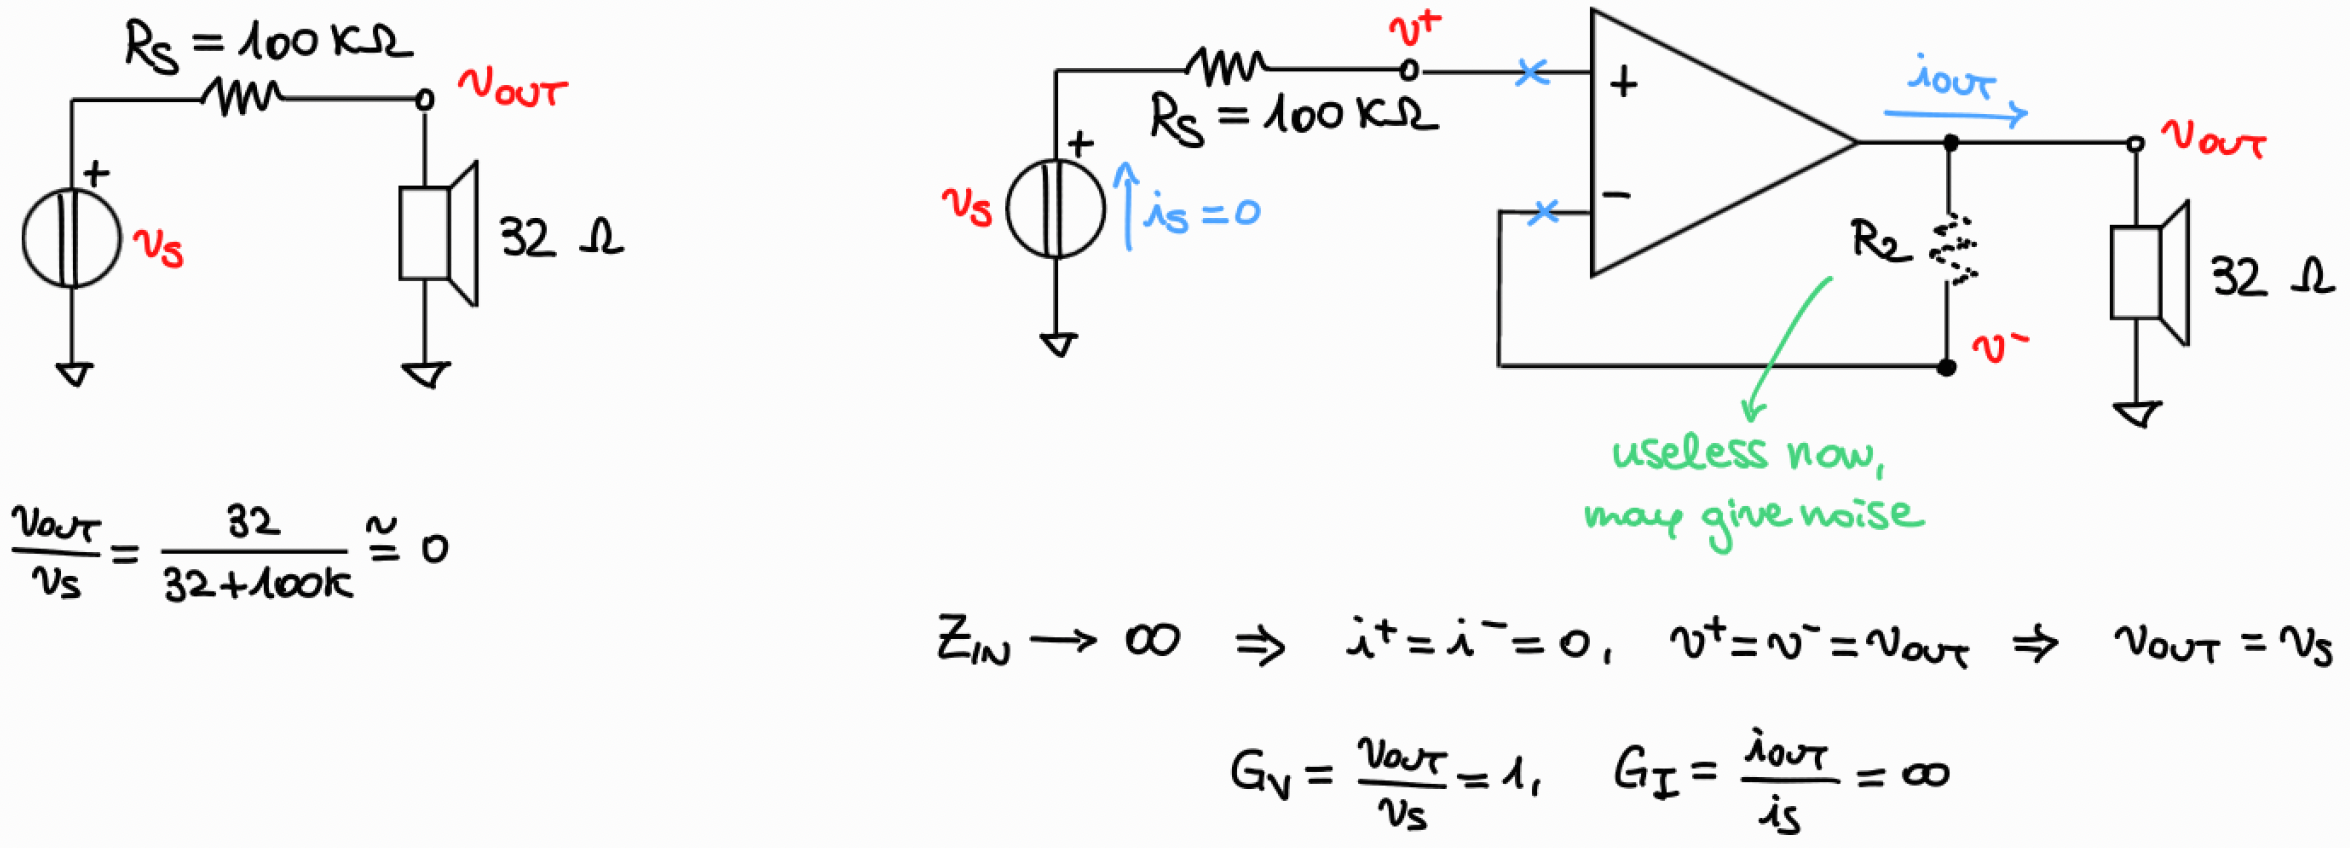
\includegraphics[width=0.90\textwidth]{Loaded_Buffer.png}
    \caption{Unity-gain buffer driving a resistive load. The voltage gain \( v_{out}/v_s = 1 \) is preserved independent of the load because the Op-Amp absorbs the current demand, decoupling source and load}
    \label{fig:loadedBuffer}
\end{figure}

\subsection{Generalizing to Impedances}
\label{ssc:261}

The resistive feedback network can be replaced by arbitrary impedances \( Z_1 \) and \( Z_2 \) to realize frequency-selective gain characteristics such as equalizers, integrators and filters. The topology of the two fundamental configurations, non-inverting and inverting, is distinguished by which input pin receives the source signal.

\begin{figure}[!htb]
    \centering
    \subfloat[Inverting configuration: the source is applied to the \( v^{-} \) pin through \( Z_1 \); the gain is \( v_{out}/v_{in} = -Z_2/Z_1 \)]{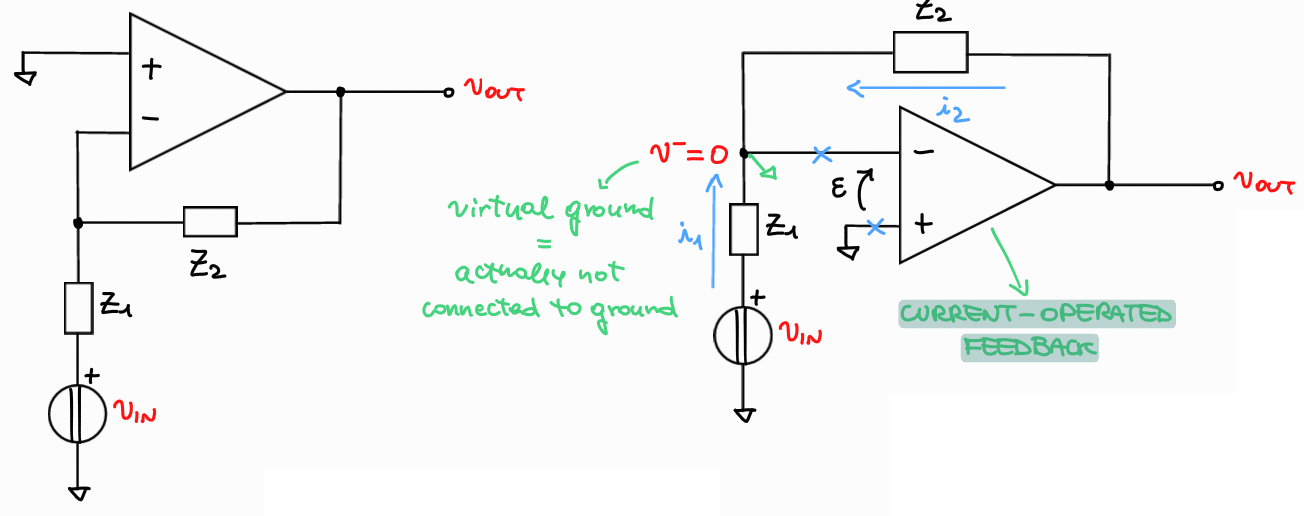
\includegraphics[height=0.15\textheight]{OPAMP_Invert_Config_Generalized.png}}
    \hfill
    \subfloat[Non-inverting configuration: the source is applied to the \( v^{+} \) pin; the gain is \( v_{out}/v_{in} = (Z_1+Z_2)/Z_1 \)]{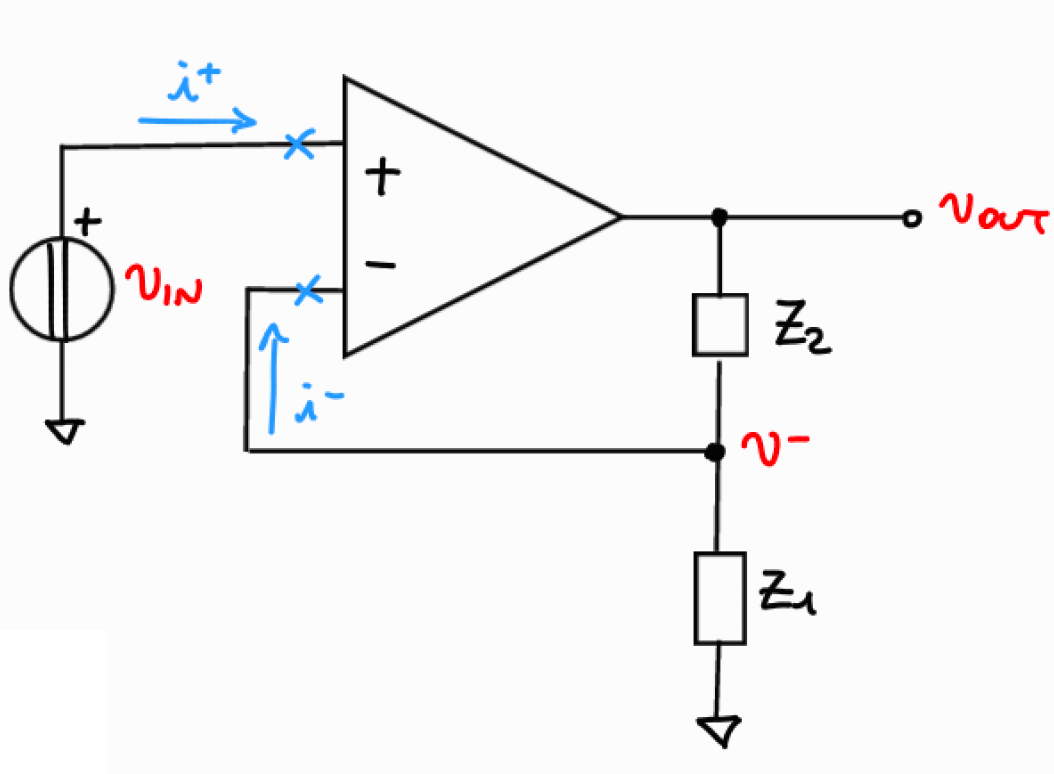
\includegraphics[height=0.15\textheight]{OPAMP_Non_Inverting_Config_Generealized.png}}
    \caption{Generalized Op-Amp configurations with complex feedback impedances \( Z_1 \) and \( Z_2 \). Replacing resistors with RC networks yields frequency-dependent gain characteristics while retaining the closed-loop gain expressions derived for the resistive case}
    \label{fig:generalizedConfigs}
\end{figure}

For the inverting configuration (figure \ref{fig:generalizedConfigs}), applying the virtual short circuit (\( v^{-} = v^{+} = 0 \)) and the zero input current condition at the inverting node gives:
\[
\frac{v_{in}}{Z_1} + \frac{v_{out}}{Z_2} = 0
\quad\Longrightarrow\quad
\frac{v_{out}}{v_{in}} = -\frac{Z_2}{Z_1}
\]
For the non-inverting configuration (figure \ref{fig:generalizedConfigs}), the virtual short circuit imposes \( v^{-} = v^{+} = v_{in} \) and the voltage divider at the inverting node gives:
\[
v^{-} = v_{out} \frac{Z_1}{Z_1 + Z_2} = v_{in}
\quad\Longrightarrow\quad
\frac{v_{out}}{v_{in}} = \frac{Z_1 + Z_2}{Z_1}
\]
These two formulas are the starting point for the analysis of virtually every linear Op-Amp circuit.